% Options for packages loaded elsewhere
\PassOptionsToPackage{unicode}{hyperref}
\PassOptionsToPackage{hyphens}{url}
\PassOptionsToPackage{dvipsnames,svgnames,x11names}{xcolor}
%
\documentclass[
  letterpaper,
  DIV=11,
  numbers=noendperiod]{scrartcl}

\usepackage{amsmath,amssymb}
\usepackage{iftex}
\ifPDFTeX
  \usepackage[T1]{fontenc}
  \usepackage[utf8]{inputenc}
  \usepackage{textcomp} % provide euro and other symbols
\else % if luatex or xetex
  \usepackage{unicode-math}
  \defaultfontfeatures{Scale=MatchLowercase}
  \defaultfontfeatures[\rmfamily]{Ligatures=TeX,Scale=1}
\fi
\usepackage{lmodern}
\ifPDFTeX\else  
    % xetex/luatex font selection
\fi
% Use upquote if available, for straight quotes in verbatim environments
\IfFileExists{upquote.sty}{\usepackage{upquote}}{}
\IfFileExists{microtype.sty}{% use microtype if available
  \usepackage[]{microtype}
  \UseMicrotypeSet[protrusion]{basicmath} % disable protrusion for tt fonts
}{}
\makeatletter
\@ifundefined{KOMAClassName}{% if non-KOMA class
  \IfFileExists{parskip.sty}{%
    \usepackage{parskip}
  }{% else
    \setlength{\parindent}{0pt}
    \setlength{\parskip}{6pt plus 2pt minus 1pt}}
}{% if KOMA class
  \KOMAoptions{parskip=half}}
\makeatother
\usepackage{xcolor}
\setlength{\emergencystretch}{3em} % prevent overfull lines
\setcounter{secnumdepth}{-\maxdimen} % remove section numbering
% Make \paragraph and \subparagraph free-standing
\makeatletter
\ifx\paragraph\undefined\else
  \let\oldparagraph\paragraph
  \renewcommand{\paragraph}{
    \@ifstar
      \xxxParagraphStar
      \xxxParagraphNoStar
  }
  \newcommand{\xxxParagraphStar}[1]{\oldparagraph*{#1}\mbox{}}
  \newcommand{\xxxParagraphNoStar}[1]{\oldparagraph{#1}\mbox{}}
\fi
\ifx\subparagraph\undefined\else
  \let\oldsubparagraph\subparagraph
  \renewcommand{\subparagraph}{
    \@ifstar
      \xxxSubParagraphStar
      \xxxSubParagraphNoStar
  }
  \newcommand{\xxxSubParagraphStar}[1]{\oldsubparagraph*{#1}\mbox{}}
  \newcommand{\xxxSubParagraphNoStar}[1]{\oldsubparagraph{#1}\mbox{}}
\fi
\makeatother


\providecommand{\tightlist}{%
  \setlength{\itemsep}{0pt}\setlength{\parskip}{0pt}}\usepackage{longtable,booktabs,array}
\usepackage{calc} % for calculating minipage widths
% Correct order of tables after \paragraph or \subparagraph
\usepackage{etoolbox}
\makeatletter
\patchcmd\longtable{\par}{\if@noskipsec\mbox{}\fi\par}{}{}
\makeatother
% Allow footnotes in longtable head/foot
\IfFileExists{footnotehyper.sty}{\usepackage{footnotehyper}}{\usepackage{footnote}}
\makesavenoteenv{longtable}
\usepackage{graphicx}
\makeatletter
\def\maxwidth{\ifdim\Gin@nat@width>\linewidth\linewidth\else\Gin@nat@width\fi}
\def\maxheight{\ifdim\Gin@nat@height>\textheight\textheight\else\Gin@nat@height\fi}
\makeatother
% Scale images if necessary, so that they will not overflow the page
% margins by default, and it is still possible to overwrite the defaults
% using explicit options in \includegraphics[width, height, ...]{}
\setkeys{Gin}{width=\maxwidth,height=\maxheight,keepaspectratio}
% Set default figure placement to htbp
\makeatletter
\def\fps@figure{htbp}
\makeatother

\usepackage{booktabs}
\usepackage{longtable}
\usepackage{array}
\usepackage{multirow}
\usepackage{wrapfig}
\usepackage{float}
\usepackage{colortbl}
\usepackage{pdflscape}
\usepackage{tabu}
\usepackage{threeparttable}
\usepackage{threeparttablex}
\usepackage[normalem]{ulem}
\usepackage{makecell}
\usepackage{xcolor}
\KOMAoption{captions}{tableheading}
\makeatletter
\@ifpackageloaded{caption}{}{\usepackage{caption}}
\AtBeginDocument{%
\ifdefined\contentsname
  \renewcommand*\contentsname{Table of contents}
\else
  \newcommand\contentsname{Table of contents}
\fi
\ifdefined\listfigurename
  \renewcommand*\listfigurename{List of Figures}
\else
  \newcommand\listfigurename{List of Figures}
\fi
\ifdefined\listtablename
  \renewcommand*\listtablename{List of Tables}
\else
  \newcommand\listtablename{List of Tables}
\fi
\ifdefined\figurename
  \renewcommand*\figurename{Figure}
\else
  \newcommand\figurename{Figure}
\fi
\ifdefined\tablename
  \renewcommand*\tablename{Table}
\else
  \newcommand\tablename{Table}
\fi
}
\@ifpackageloaded{float}{}{\usepackage{float}}
\floatstyle{ruled}
\@ifundefined{c@chapter}{\newfloat{codelisting}{h}{lop}}{\newfloat{codelisting}{h}{lop}[chapter]}
\floatname{codelisting}{Listing}
\newcommand*\listoflistings{\listof{codelisting}{List of Listings}}
\makeatother
\makeatletter
\makeatother
\makeatletter
\@ifpackageloaded{caption}{}{\usepackage{caption}}
\@ifpackageloaded{subcaption}{}{\usepackage{subcaption}}
\makeatother

\ifLuaTeX
  \usepackage{selnolig}  % disable illegal ligatures
\fi
\usepackage{bookmark}

\IfFileExists{xurl.sty}{\usepackage{xurl}}{} % add URL line breaks if available
\urlstyle{same} % disable monospaced font for URLs
\hypersetup{
  pdftitle={Relatório Temas para a Saúde},
  colorlinks=true,
  linkcolor={blue},
  filecolor={Maroon},
  citecolor={Blue},
  urlcolor={Blue},
  pdfcreator={LaTeX via pandoc}}


\title{Relatório Temas para a Saúde}
\author{}
\date{}

\begin{document}
\maketitle


\section{Análise Exploratória e
descritiva}\label{anuxe1lise-exploratuxf3ria-e-descritiva}

\subsection{Agravos negligenciados}\label{agravos-negligenciados}

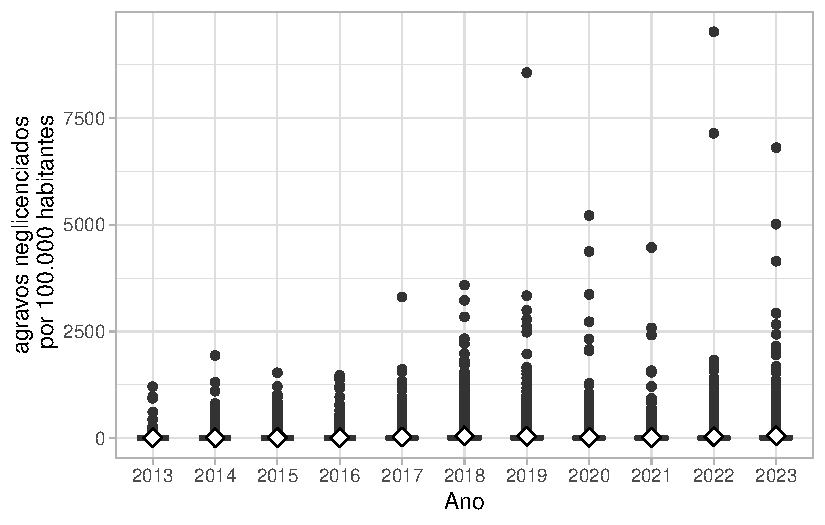
\includegraphics{Relatório_files/figure-pdf/unnamed-chunk-5-1.pdf}

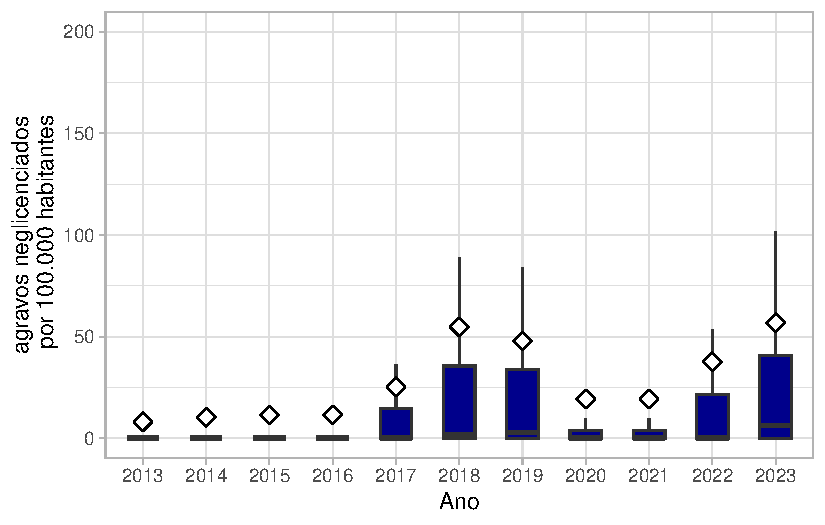
\includegraphics{Relatório_files/figure-pdf/unnamed-chunk-6-1.pdf}

\begin{longtable}[]{@{}
  >{\raggedright\arraybackslash}p{(\columnwidth - 16\tabcolsep) * \real{0.0575}}
  >{\raggedleft\arraybackslash}p{(\columnwidth - 16\tabcolsep) * \real{0.1149}}
  >{\raggedleft\arraybackslash}p{(\columnwidth - 16\tabcolsep) * \real{0.1609}}
  >{\raggedleft\arraybackslash}p{(\columnwidth - 16\tabcolsep) * \real{0.1034}}
  >{\raggedleft\arraybackslash}p{(\columnwidth - 16\tabcolsep) * \real{0.1149}}
  >{\raggedleft\arraybackslash}p{(\columnwidth - 16\tabcolsep) * \real{0.0920}}
  >{\raggedleft\arraybackslash}p{(\columnwidth - 16\tabcolsep) * \real{0.1149}}
  >{\raggedleft\arraybackslash}p{(\columnwidth - 16\tabcolsep) * \real{0.1264}}
  >{\raggedleft\arraybackslash}p{(\columnwidth - 16\tabcolsep) * \real{0.1149}}@{}}
\toprule\noalign{}
\begin{minipage}[b]{\linewidth}\raggedright
ano
\end{minipage} & \begin{minipage}[b]{\linewidth}\raggedleft
média
\end{minipage} & \begin{minipage}[b]{\linewidth}\raggedleft
desvio padrão
\end{minipage} & \begin{minipage}[b]{\linewidth}\raggedleft
máximo
\end{minipage} & \begin{minipage}[b]{\linewidth}\raggedleft
1\_quartil
\end{minipage} & \begin{minipage}[b]{\linewidth}\raggedleft
mediana
\end{minipage} & \begin{minipage}[b]{\linewidth}\raggedleft
3\_quartil
\end{minipage} & \begin{minipage}[b]{\linewidth}\raggedleft
assimetria
\end{minipage} & \begin{minipage}[b]{\linewidth}\raggedleft
curtose
\end{minipage} \\
\midrule\noalign{}
\endhead
\bottomrule\noalign{}
\endlastfoot
2013 & 8.047367 & 64.93441 & 1206.950 & 0 & 0.0000 & 0.00000 & 13.598703
& 209.4852 \\
2014 & 10.286001 & 68.91488 & 1937.473 & 0 & 0.0000 & 0.00000 &
15.624793 & 328.3808 \\
2015 & 11.467288 & 62.82786 & 1531.931 & 0 & 0.0000 & 0.00000 &
11.447381 & 180.6773 \\
2016 & 11.464230 & 68.88173 & 1470.085 & 0 & 0.0000 & 0.00000 &
13.319916 & 223.7612 \\
2017 & 25.254745 & 94.50434 & 3308.350 & 0 & 0.0000 & 14.49280 &
13.494733 & 333.8131 \\
2018 & 54.749720 & 168.43575 & 3585.230 & 0 & 1.7051 & 35.55240 &
8.278695 & 110.3641 \\
2019 & 47.861453 & 186.95398 & 8564.232 & 0 & 2.8986 & 33.63462 &
22.374227 & 858.2109 \\
2020 & 19.280703 & 143.27272 & 5217.391 & 0 & 0.0000 & 3.81215 &
22.516193 & 650.7542 \\
2021 & 19.277594 & 110.78424 & 4467.354 & 0 & 0.0000 & 3.79820 &
20.787160 & 655.1030 \\
2022 & 37.625804 & 196.20056 & 9521.554 & 0 & 0.0000 & 21.33790 &
31.131295 & 1339.6693 \\
2023 & 56.829860 & 203.94840 & 6804.669 & 0 & 6.3217 & 40.71213 &
14.672786 & 352.0877 \\
\end{longtable}

\begin{longtable}[]{@{}lr@{}}
\caption{10 UFs com maior média de agravos por 100.000
habitantes}\tabularnewline
\toprule\noalign{}
UF & Média Agravo \\
\midrule\noalign{}
\endfirsthead
\toprule\noalign{}
UF & Média Agravo \\
\midrule\noalign{}
\endhead
\bottomrule\noalign{}
\endlastfoot
AM & 94.62655 \\
AL & 89.88990 \\
MG & 46.81703 \\
PE & 46.61969 \\
CE & 42.35827 \\
MT & 41.91309 \\
MA & 35.30984 \\
PA & 32.81917 \\
TO & 32.20780 \\
PI & 31.52319 \\
\end{longtable}

\subsection{Alimentação saudável}\label{alimentauxe7uxe3o-sauduxe1vel}

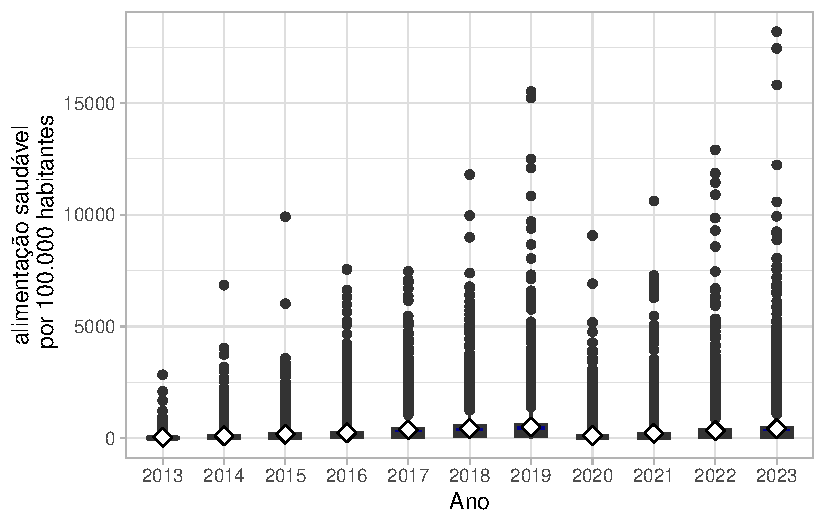
\includegraphics{Relatório_files/figure-pdf/unnamed-chunk-9-1.pdf}

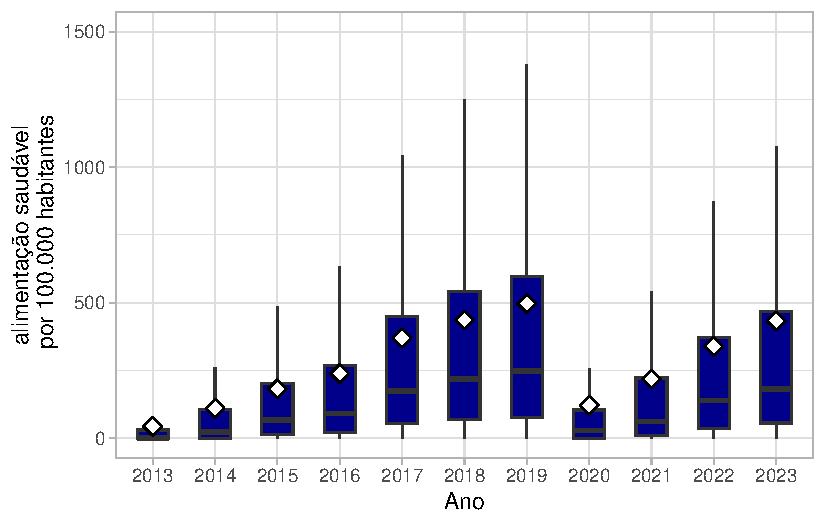
\includegraphics{Relatório_files/figure-pdf/unnamed-chunk-10-1.pdf}

\begin{longtable}[]{@{}
  >{\raggedright\arraybackslash}p{(\columnwidth - 16\tabcolsep) * \real{0.0562}}
  >{\raggedleft\arraybackslash}p{(\columnwidth - 16\tabcolsep) * \real{0.1124}}
  >{\raggedleft\arraybackslash}p{(\columnwidth - 16\tabcolsep) * \real{0.1573}}
  >{\raggedleft\arraybackslash}p{(\columnwidth - 16\tabcolsep) * \real{0.1124}}
  >{\raggedleft\arraybackslash}p{(\columnwidth - 16\tabcolsep) * \real{0.1124}}
  >{\raggedleft\arraybackslash}p{(\columnwidth - 16\tabcolsep) * \real{0.1011}}
  >{\raggedleft\arraybackslash}p{(\columnwidth - 16\tabcolsep) * \real{0.1124}}
  >{\raggedleft\arraybackslash}p{(\columnwidth - 16\tabcolsep) * \real{0.1236}}
  >{\raggedleft\arraybackslash}p{(\columnwidth - 16\tabcolsep) * \real{0.1124}}@{}}
\toprule\noalign{}
\begin{minipage}[b]{\linewidth}\raggedright
ano
\end{minipage} & \begin{minipage}[b]{\linewidth}\raggedleft
média
\end{minipage} & \begin{minipage}[b]{\linewidth}\raggedleft
desvio padrão
\end{minipage} & \begin{minipage}[b]{\linewidth}\raggedleft
máximo
\end{minipage} & \begin{minipage}[b]{\linewidth}\raggedleft
1\_quartil
\end{minipage} & \begin{minipage}[b]{\linewidth}\raggedleft
mediana
\end{minipage} & \begin{minipage}[b]{\linewidth}\raggedleft
3\_quartil
\end{minipage} & \begin{minipage}[b]{\linewidth}\raggedleft
assimetria
\end{minipage} & \begin{minipage}[b]{\linewidth}\raggedleft
curtose
\end{minipage} \\
\midrule\noalign{}
\endhead
\bottomrule\noalign{}
\endlastfoot
2013 & 43.41202 & 149.9152 & 2836.756 & 0.00000 & 0.0000 & 30.2810 &
10.089878 & 146.36135 \\
2014 & 110.45384 & 287.9461 & 6843.201 & 0.00000 & 22.8363 & 105.1830 &
9.259979 & 148.65955 \\
2015 & 182.04111 & 362.9468 & 9907.765 & 12.66430 & 66.4105 & 202.5091 &
8.148170 & 148.28940 \\
2016 & 238.73776 & 475.0052 & 7558.860 & 22.04162 & 91.5262 & 267.7193 &
6.292101 & 64.00350 \\
2017 & 369.96409 & 582.6465 & 7462.687 & 53.87820 & 173.9635 & 449.9241
& 4.328180 & 32.38542 \\
2018 & 436.15208 & 677.7487 & 11797.101 & 69.56930 & 218.9490 & 542.4837
& 4.984800 & 47.03372 \\
2019 & 496.99954 & 837.0470 & 15514.443 & 75.78630 & 247.2601 & 597.6826
& 6.378766 & 74.99904 \\
2020 & 121.04649 & 339.8253 & 9072.464 & 0.00000 & 28.9855 & 103.8461 &
10.306067 & 178.25084 \\
2021 & 218.12093 & 498.7237 & 10610.080 & 9.65160 & 61.2404 & 221.8388 &
7.616492 & 96.43906 \\
2022 & 339.34837 & 687.3535 & 12902.085 & 36.11585 & 138.5390 & 371.6102
& 7.467299 & 92.45209 \\
2023 & 432.87282 & 880.6483 & 18189.421 & 56.43543 & 182.1289 & 466.1863
& 7.825814 & 105.01722 \\
\end{longtable}

\begin{longtable}[]{@{}lr@{}}
\caption{10 UFs com maior média de alimentacao por 100.000
habitantes}\tabularnewline
\toprule\noalign{}
UF & Média alimentacao \\
\midrule\noalign{}
\endfirsthead
\toprule\noalign{}
UF & Média alimentacao \\
\midrule\noalign{}
\endhead
\bottomrule\noalign{}
\endlastfoot
AL & 542.7067 \\
MG & 539.7857 \\
AM & 388.0099 \\
RS & 366.4856 \\
GO & 361.7034 \\
TO & 322.2241 \\
PI & 313.1994 \\
PE & 303.1462 \\
PB & 280.8006 \\
CE & 265.0042 \\
\end{longtable}

\subsection{Autocuidado de pessoas com
doenças}\label{autocuidado-de-pessoas-com-doenuxe7as}

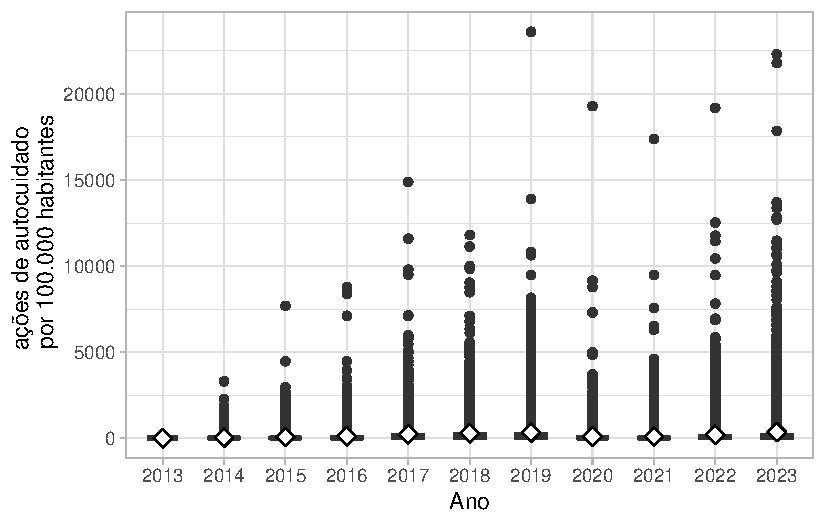
\includegraphics{Relatório_files/figure-pdf/unnamed-chunk-13-1.pdf}

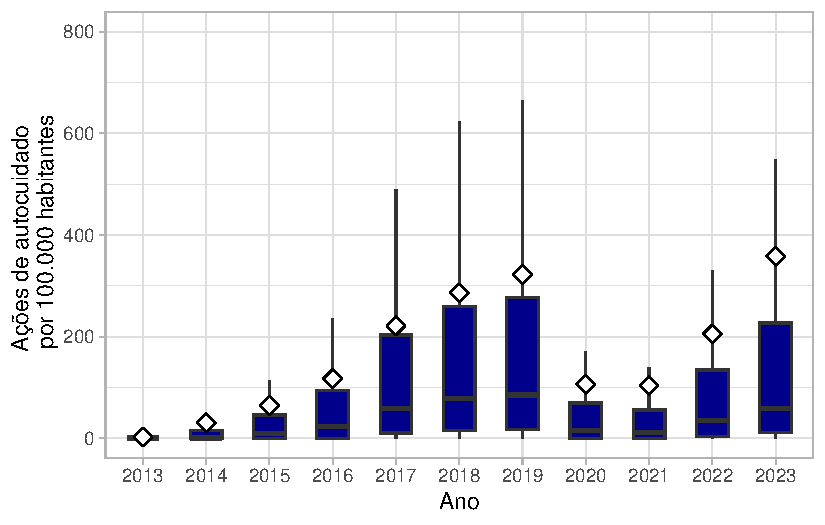
\includegraphics{Relatório_files/figure-pdf/unnamed-chunk-14-1.pdf}

\begin{longtable}[]{@{}
  >{\raggedright\arraybackslash}p{(\columnwidth - 16\tabcolsep) * \real{0.0549}}
  >{\raggedleft\arraybackslash}p{(\columnwidth - 16\tabcolsep) * \real{0.1209}}
  >{\raggedleft\arraybackslash}p{(\columnwidth - 16\tabcolsep) * \real{0.1538}}
  >{\raggedleft\arraybackslash}p{(\columnwidth - 16\tabcolsep) * \real{0.1209}}
  >{\raggedleft\arraybackslash}p{(\columnwidth - 16\tabcolsep) * \real{0.1099}}
  >{\raggedleft\arraybackslash}p{(\columnwidth - 16\tabcolsep) * \real{0.0989}}
  >{\raggedleft\arraybackslash}p{(\columnwidth - 16\tabcolsep) * \real{0.1099}}
  >{\raggedleft\arraybackslash}p{(\columnwidth - 16\tabcolsep) * \real{0.1209}}
  >{\raggedleft\arraybackslash}p{(\columnwidth - 16\tabcolsep) * \real{0.1099}}@{}}
\toprule\noalign{}
\begin{minipage}[b]{\linewidth}\raggedright
ano
\end{minipage} & \begin{minipage}[b]{\linewidth}\raggedleft
média
\end{minipage} & \begin{minipage}[b]{\linewidth}\raggedleft
desvio padrão
\end{minipage} & \begin{minipage}[b]{\linewidth}\raggedleft
máximo
\end{minipage} & \begin{minipage}[b]{\linewidth}\raggedleft
1\_quartil
\end{minipage} & \begin{minipage}[b]{\linewidth}\raggedleft
mediana
\end{minipage} & \begin{minipage}[b]{\linewidth}\raggedleft
3\_quartil
\end{minipage} & \begin{minipage}[b]{\linewidth}\raggedleft
assimetria
\end{minipage} & \begin{minipage}[b]{\linewidth}\raggedleft
curtose
\end{minipage} \\
\midrule\noalign{}
\endhead
\bottomrule\noalign{}
\endlastfoot
2013 & 2.144704 & 13.61635 & 212.5809 & 0.00000 & 0.00000 & 0.00000 &
10.754716 & 139.13681 \\
2014 & 30.366427 & 124.47758 & 3302.5885 & 0.00000 & 0.00000 & 15.34790
& 12.852869 & 249.20855 \\
2015 & 64.639629 & 224.23628 & 7684.9577 & 0.00000 & 8.91870 & 45.63160
& 14.461698 & 367.90274 \\
2016 & 117.319435 & 364.45937 & 8782.6087 & 0.00000 & 23.18980 &
94.41220 & 11.824437 & 220.93390 \\
2017 & 221.331515 & 590.80704 & 14881.2192 & 10.08330 & 58.19030 &
202.92245 & 9.906361 & 159.90419 \\
2018 & 285.976424 & 679.08245 & 11803.8741 & 15.12785 & 78.02340 &
258.72425 & 6.933803 & 76.10121 \\
2019 & 322.531905 & 836.51417 & 23614.6096 & 17.04030 & 85.09085 &
276.64528 & 9.151992 & 158.36463 \\
2020 & 106.352692 & 447.44912 & 19289.3401 & 0.00000 & 15.05340 &
69.24395 & 21.974974 & 777.67099 \\
2021 & 103.806886 & 451.72758 & 17385.7868 & 0.00000 & 10.90870 &
55.40020 & 17.512418 & 513.08651 \\
2022 & 205.208041 & 692.65672 & 19184.7585 & 3.61240 & 35.14000 &
134.29330 & 11.102500 & 196.32079 \\
2023 & 358.156470 & 1103.97478 & 22307.9621 & 11.55415 & 58.66535 &
226.63640 & 8.243767 & 104.58803 \\
\end{longtable}

\begin{longtable}[]{@{}lr@{}}
\caption{10 UFs com maior média de ações de autocuidado por 100.000
habitantes}\tabularnewline
\toprule\noalign{}
UF & Média Autocuidado \\
\midrule\noalign{}
\endfirsthead
\toprule\noalign{}
UF & Média Autocuidado \\
\midrule\noalign{}
\endhead
\bottomrule\noalign{}
\endlastfoot
MG & 388.6747 \\
SC & 247.2616 \\
GO & 243.0693 \\
RS & 232.7296 \\
TO & 215.7645 \\
AL & 190.7134 \\
SP & 189.8866 \\
MT & 162.5645 \\
PI & 151.2948 \\
MS & 136.1506 \\
\end{longtable}

\subsection{Ações de combate ao Aedes
aegypt}\label{auxe7uxf5es-de-combate-ao-aedes-aegypt}

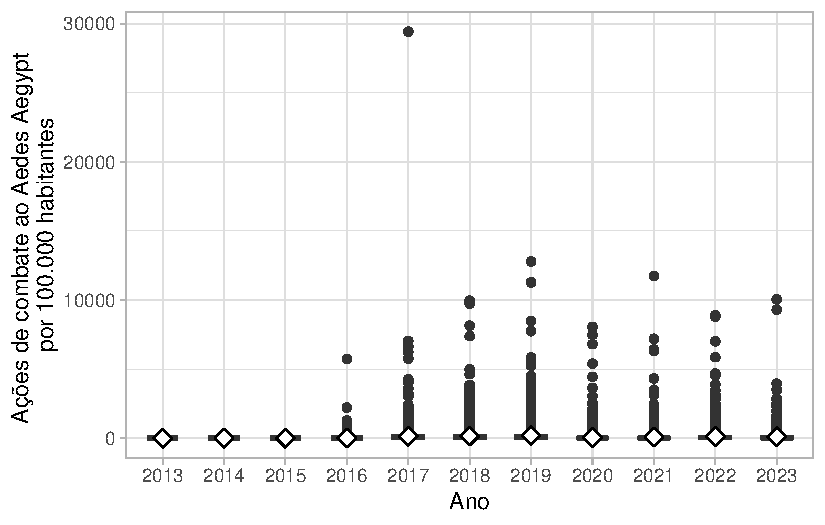
\includegraphics{Relatório_files/figure-pdf/unnamed-chunk-17-1.pdf}

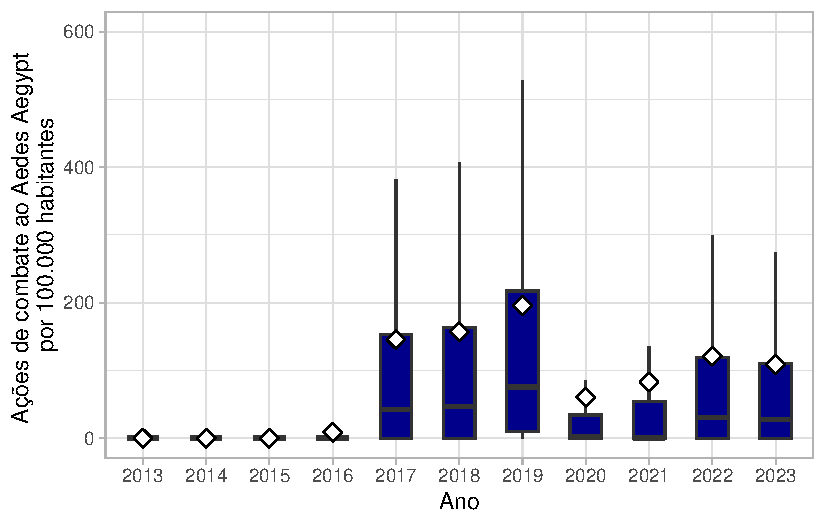
\includegraphics{Relatório_files/figure-pdf/unnamed-chunk-18-1.pdf}

\begin{longtable}[]{@{}
  >{\raggedright\arraybackslash}p{(\columnwidth - 16\tabcolsep) * \real{0.0549}}
  >{\raggedleft\arraybackslash}p{(\columnwidth - 16\tabcolsep) * \real{0.1319}}
  >{\raggedleft\arraybackslash}p{(\columnwidth - 16\tabcolsep) * \real{0.1538}}
  >{\raggedleft\arraybackslash}p{(\columnwidth - 16\tabcolsep) * \real{0.1209}}
  >{\raggedleft\arraybackslash}p{(\columnwidth - 16\tabcolsep) * \real{0.1099}}
  >{\raggedleft\arraybackslash}p{(\columnwidth - 16\tabcolsep) * \real{0.0879}}
  >{\raggedleft\arraybackslash}p{(\columnwidth - 16\tabcolsep) * \real{0.1099}}
  >{\raggedleft\arraybackslash}p{(\columnwidth - 16\tabcolsep) * \real{0.1209}}
  >{\raggedleft\arraybackslash}p{(\columnwidth - 16\tabcolsep) * \real{0.1099}}@{}}
\toprule\noalign{}
\begin{minipage}[b]{\linewidth}\raggedright
ano
\end{minipage} & \begin{minipage}[b]{\linewidth}\raggedleft
média
\end{minipage} & \begin{minipage}[b]{\linewidth}\raggedleft
desvio padrão
\end{minipage} & \begin{minipage}[b]{\linewidth}\raggedleft
máximo
\end{minipage} & \begin{minipage}[b]{\linewidth}\raggedleft
1\_quartil
\end{minipage} & \begin{minipage}[b]{\linewidth}\raggedleft
mediana
\end{minipage} & \begin{minipage}[b]{\linewidth}\raggedleft
3\_quartil
\end{minipage} & \begin{minipage}[b]{\linewidth}\raggedleft
assimetria
\end{minipage} & \begin{minipage}[b]{\linewidth}\raggedleft
curtose
\end{minipage} \\
\midrule\noalign{}
\endhead
\bottomrule\noalign{}
\endlastfoot
2013 & 0.0000000 & 0.0000000 & 0.0000 & 0.0000 & 0.0000 & 0.0000 & NaN &
NaN \\
2014 & 0.0000000 & 0.0000000 & 0.0000 & 0.0000 & 0.0000 & 0.0000 & NaN &
NaN \\
2015 & 0.0045401 & 0.2903237 & 19.3255 & 0.0000 & 0.0000 & 0.0000 &
66.42538 & 4420.7615 \\
2016 & 8.5917759 & 100.7306415 & 5740.8844 & 0.0000 & 0.0000 & 0.0000 &
40.69572 & 2143.9396 \\
2017 & 145.4603232 & 511.0370120 & 29409.1114 & 0.0000 & 42.0433 &
152.9415 & 37.09565 & 2020.9686 \\
2018 & 156.9949706 & 388.3161002 & 9950.3517 & 0.0000 & 46.3795 &
163.2743 & 11.30401 & 219.6703 \\
2019 & 195.7307786 & 456.0882216 & 12783.3753 & 9.6623 & 75.8659 &
217.3913 & 11.46453 & 229.2798 \\
2020 & 60.5595283 & 273.9444770 & 8058.3756 & 0.0000 & 1.6103 & 34.3471
& 16.79875 & 393.6703 \\
2021 & 82.8450328 & 323.6387937 & 11738.5787 & 0.0000 & 0.0000 & 54.6523
& 16.95168 & 460.5217 \\
2022 & 121.1576904 & 333.8113667 & 8903.1339 & 0.0000 & 30.2847 &
119.5536 & 12.36150 & 250.6772 \\
2023 & 108.8240598 & 290.7923964 & 10037.6117 & 0.0000 & 28.0047 &
109.8249 & 15.91379 & 456.2393 \\
\end{longtable}

\begin{longtable}[]{@{}lr@{}}
\caption{10 UFs com maior média de Ações de combate ao Aedes Aegypt por
100.000 habitantes}\tabularnewline
\toprule\noalign{}
UF & Média Ações \\
\midrule\noalign{}
\endfirsthead
\toprule\noalign{}
UF & Média Ações \\
\midrule\noalign{}
\endhead
\bottomrule\noalign{}
\endlastfoot
AL & 187.39116 \\
RS & 167.70391 \\
AM & 142.89538 \\
GO & 136.37930 \\
MT & 126.33296 \\
CE & 109.88190 \\
RO & 108.35433 \\
MG & 108.18938 \\
TO & 95.90684 \\
MA & 84.76395 \\
\end{longtable}

\subsection{Cidadania e direitos
humanos}\label{cidadania-e-direitos-humanos}

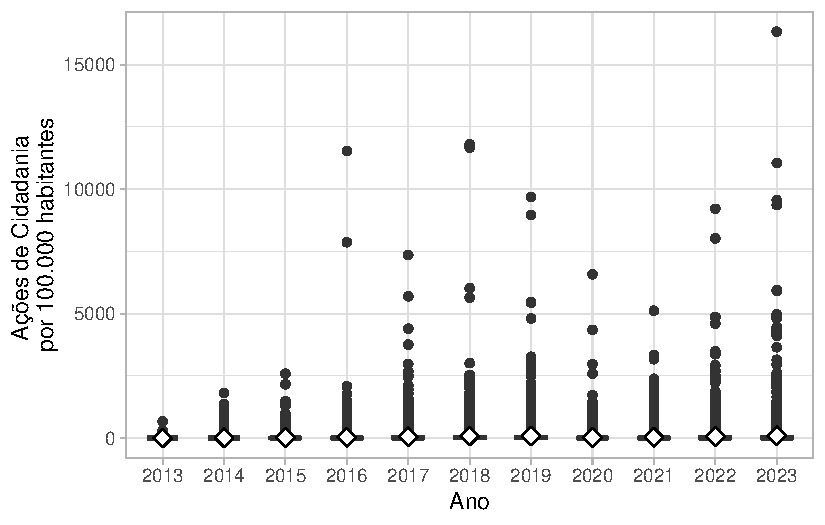
\includegraphics{Relatório_files/figure-pdf/unnamed-chunk-21-1.pdf}

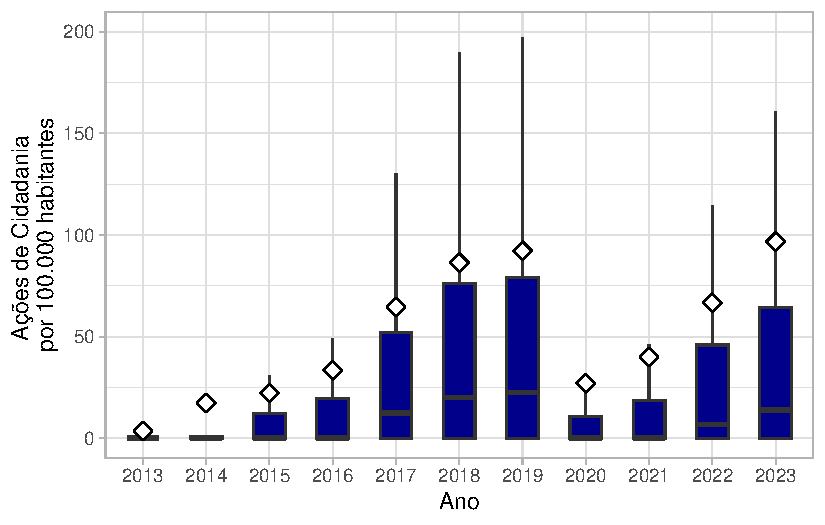
\includegraphics{Relatório_files/figure-pdf/unnamed-chunk-22-1.pdf}

\begin{longtable}[]{@{}
  >{\raggedright\arraybackslash}p{(\columnwidth - 16\tabcolsep) * \real{0.0556}}
  >{\raggedleft\arraybackslash}p{(\columnwidth - 16\tabcolsep) * \real{0.1111}}
  >{\raggedleft\arraybackslash}p{(\columnwidth - 16\tabcolsep) * \real{0.1556}}
  >{\raggedleft\arraybackslash}p{(\columnwidth - 16\tabcolsep) * \real{0.1222}}
  >{\raggedleft\arraybackslash}p{(\columnwidth - 16\tabcolsep) * \real{0.1111}}
  >{\raggedleft\arraybackslash}p{(\columnwidth - 16\tabcolsep) * \real{0.1000}}
  >{\raggedleft\arraybackslash}p{(\columnwidth - 16\tabcolsep) * \real{0.1111}}
  >{\raggedleft\arraybackslash}p{(\columnwidth - 16\tabcolsep) * \real{0.1222}}
  >{\raggedleft\arraybackslash}p{(\columnwidth - 16\tabcolsep) * \real{0.1111}}@{}}
\toprule\noalign{}
\begin{minipage}[b]{\linewidth}\raggedright
ano
\end{minipage} & \begin{minipage}[b]{\linewidth}\raggedleft
média
\end{minipage} & \begin{minipage}[b]{\linewidth}\raggedleft
desvio padrão
\end{minipage} & \begin{minipage}[b]{\linewidth}\raggedleft
máximo
\end{minipage} & \begin{minipage}[b]{\linewidth}\raggedleft
1\_quartil
\end{minipage} & \begin{minipage}[b]{\linewidth}\raggedleft
mediana
\end{minipage} & \begin{minipage}[b]{\linewidth}\raggedleft
3\_quartil
\end{minipage} & \begin{minipage}[b]{\linewidth}\raggedleft
assimetria
\end{minipage} & \begin{minipage}[b]{\linewidth}\raggedleft
curtose
\end{minipage} \\
\midrule\noalign{}
\endhead
\bottomrule\noalign{}
\endlastfoot
2013 & 3.501147 & 27.51691 & 673.0041 & 0 & 0.00000 & 0.00000 & 15.60148
& 317.9481 \\
2014 & 17.295434 & 80.70371 & 1813.0841 & 0 & 0.00000 & 0.56840 &
11.42443 & 181.5006 \\
2015 & 22.278181 & 99.07697 & 2586.8179 & 0 & 0.00000 & 12.30495 &
13.34039 & 251.3823 \\
2016 & 33.428513 & 221.60261 & 11536.7679 & 0 & 0.00000 & 19.53235 &
37.32604 & 1752.5318 \\
2017 & 64.553999 & 222.55461 & 7356.1544 & 0 & 12.44560 & 52.12935 &
14.85905 & 356.7977 \\
2018 & 86.435284 & 316.26798 & 11797.1014 & 0 & 19.92880 & 76.04560 &
22.16446 & 731.2456 \\
2019 & 92.197135 & 302.14490 & 9681.1594 & 0 & 22.45720 & 78.93098 &
15.73113 & 390.3788 \\
2020 & 27.028776 & 155.98416 & 6581.0594 & 0 & 0.00000 & 10.48660 &
23.58892 & 809.4169 \\
2021 & 39.925128 & 170.73861 & 5119.8114 & 0 & 0.00000 & 18.40940 &
13.34659 & 271.4396 \\
2022 & 66.586169 & 271.45234 & 9208.8740 & 0 & 6.63960 & 45.86840 &
17.31304 & 448.6741 \\
2023 & 96.706468 & 436.98220 & 16319.7336 & 0 & 13.81425 & 64.41848 &
19.29655 & 534.0297 \\
\end{longtable}

\begin{longtable}[]{@{}lr@{}}
\caption{10 UFs com maior média de Ações de Cidadania por 100.000
habitantes}\tabularnewline
\toprule\noalign{}
UF & Média Ações \\
\midrule\noalign{}
\endfirsthead
\toprule\noalign{}
UF & Média Ações \\
\midrule\noalign{}
\endhead
\bottomrule\noalign{}
\endlastfoot
AM & 114.09374 \\
MG & 97.68653 \\
AL & 89.14643 \\
GO & 80.22907 \\
RS & 76.60108 \\
TO & 73.25584 \\
MT & 63.91529 \\
RN & 56.91270 \\
CE & 51.58832 \\
PI & 50.20940 \\
\end{longtable}

\subsection{Dependência química /
tabaco}\label{dependuxeancia-quuxedmica-tabaco}

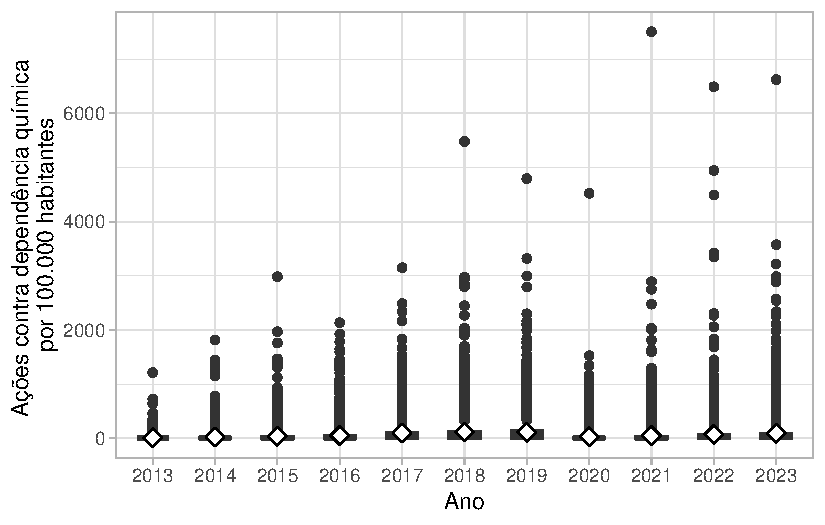
\includegraphics{Relatório_files/figure-pdf/unnamed-chunk-25-1.pdf}

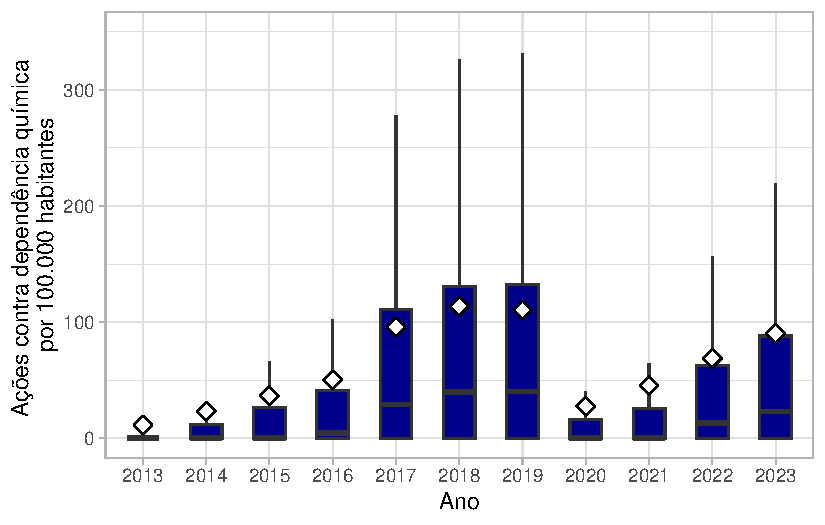
\includegraphics{Relatório_files/figure-pdf/unnamed-chunk-26-1.pdf}

\begin{longtable}[]{@{}
  >{\raggedright\arraybackslash}p{(\columnwidth - 16\tabcolsep) * \real{0.0575}}
  >{\raggedleft\arraybackslash}p{(\columnwidth - 16\tabcolsep) * \real{0.1149}}
  >{\raggedleft\arraybackslash}p{(\columnwidth - 16\tabcolsep) * \real{0.1609}}
  >{\raggedleft\arraybackslash}p{(\columnwidth - 16\tabcolsep) * \real{0.1034}}
  >{\raggedleft\arraybackslash}p{(\columnwidth - 16\tabcolsep) * \real{0.1149}}
  >{\raggedleft\arraybackslash}p{(\columnwidth - 16\tabcolsep) * \real{0.0920}}
  >{\raggedleft\arraybackslash}p{(\columnwidth - 16\tabcolsep) * \real{0.1149}}
  >{\raggedleft\arraybackslash}p{(\columnwidth - 16\tabcolsep) * \real{0.1264}}
  >{\raggedleft\arraybackslash}p{(\columnwidth - 16\tabcolsep) * \real{0.1149}}@{}}
\toprule\noalign{}
\begin{minipage}[b]{\linewidth}\raggedright
ano
\end{minipage} & \begin{minipage}[b]{\linewidth}\raggedleft
média
\end{minipage} & \begin{minipage}[b]{\linewidth}\raggedleft
desvio padrão
\end{minipage} & \begin{minipage}[b]{\linewidth}\raggedleft
máximo
\end{minipage} & \begin{minipage}[b]{\linewidth}\raggedleft
1\_quartil
\end{minipage} & \begin{minipage}[b]{\linewidth}\raggedleft
mediana
\end{minipage} & \begin{minipage}[b]{\linewidth}\raggedleft
3\_quartil
\end{minipage} & \begin{minipage}[b]{\linewidth}\raggedleft
assimetria
\end{minipage} & \begin{minipage}[b]{\linewidth}\raggedleft
curtose
\end{minipage} \\
\midrule\noalign{}
\endhead
\bottomrule\noalign{}
\endlastfoot
2013 & 11.39181 & 56.29572 & 1212.438 & 0 & 0.0000 & 0.00000 & 12.322983
& 210.51285 \\
2014 & 23.09458 & 88.69071 & 1810.358 & 0 & 0.0000 & 11.49100 &
10.034062 & 142.22011 \\
2015 & 36.51284 & 115.77356 & 2980.805 & 0 & 0.0000 & 26.49445 &
9.674480 & 157.72396 \\
2016 & 50.21627 & 133.21560 & 2134.219 & 0 & 4.4596 & 41.07408 &
6.532996 & 63.94003 \\
2017 & 95.72165 & 183.59713 & 3148.254 & 0 & 28.9855 & 111.11915 &
4.864221 & 43.50828 \\
2018 & 113.46433 & 223.90635 & 5478.261 & 0 & 39.6825 & 130.44895 &
6.894729 & 97.62544 \\
2019 & 110.34576 & 211.28564 & 4793.079 & 0 & 40.1374 & 132.58542 &
6.526499 & 85.01410 \\
2020 & 27.48349 & 106.24201 & 4521.739 & 0 & 0.0000 & 16.29155 &
19.308719 & 688.11671 \\
2021 & 45.33366 & 179.17529 & 7505.071 & 0 & 0.0000 & 25.58530 &
18.928200 & 648.58628 \\
2022 & 68.71972 & 203.70032 & 6489.815 & 0 & 12.9740 & 62.58310 &
13.985578 & 325.84198 \\
2023 & 90.14072 & 223.93235 & 6621.622 & 0 & 22.8301 & 88.02625 &
9.649270 & 182.66671 \\
\end{longtable}

\begin{longtable}[]{@{}lr@{}}
\caption{10 UFs com maior média de Ações contra dependência química por
100.000 habitantes}\tabularnewline
\toprule\noalign{}
UF & Média Ações \\
\midrule\noalign{}
\endfirsthead
\toprule\noalign{}
UF & Média Ações \\
\midrule\noalign{}
\endhead
\bottomrule\noalign{}
\endlastfoot
MG & 146.93142 \\
RS & 91.57771 \\
AM & 86.95773 \\
GO & 76.36243 \\
SC & 74.28644 \\
RO & 70.89590 \\
TO & 70.87137 \\
AL & 69.32284 \\
MT & 65.09259 \\
RN & 61.55464 \\
\end{longtable}

\subsection{Envelhecimento /
Climatério}\label{envelhecimento-climatuxe9rio}

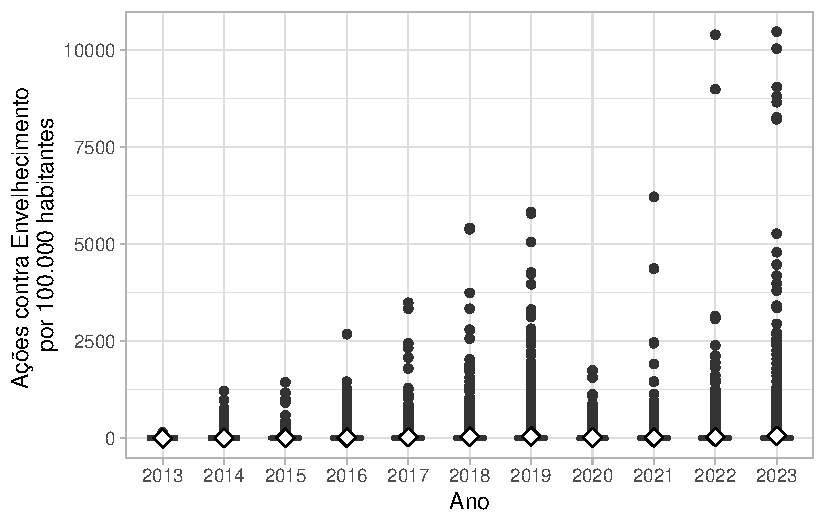
\includegraphics{Relatório_files/figure-pdf/unnamed-chunk-29-1.pdf}

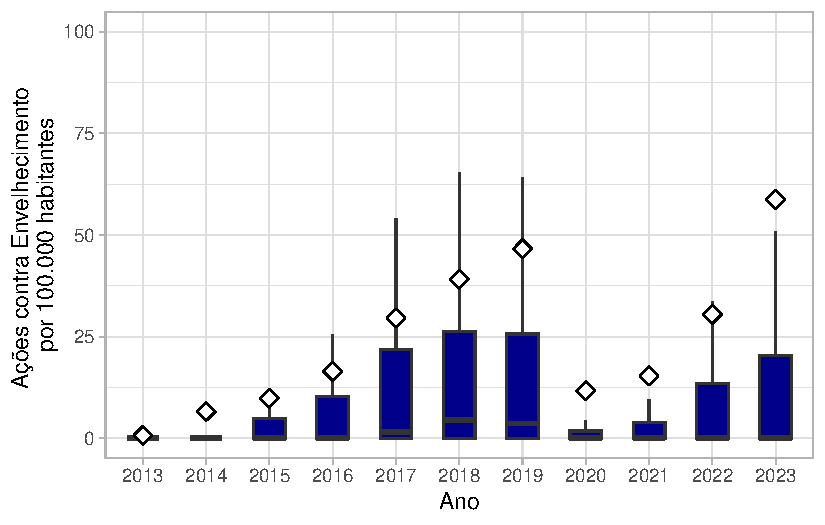
\includegraphics{Relatório_files/figure-pdf/unnamed-chunk-30-1.pdf}

\begin{longtable}[]{@{}
  >{\raggedright\arraybackslash}p{(\columnwidth - 16\tabcolsep) * \real{0.0556}}
  >{\raggedleft\arraybackslash}p{(\columnwidth - 16\tabcolsep) * \real{0.1222}}
  >{\raggedleft\arraybackslash}p{(\columnwidth - 16\tabcolsep) * \real{0.1556}}
  >{\raggedleft\arraybackslash}p{(\columnwidth - 16\tabcolsep) * \real{0.1222}}
  >{\raggedleft\arraybackslash}p{(\columnwidth - 16\tabcolsep) * \real{0.1111}}
  >{\raggedleft\arraybackslash}p{(\columnwidth - 16\tabcolsep) * \real{0.0889}}
  >{\raggedleft\arraybackslash}p{(\columnwidth - 16\tabcolsep) * \real{0.1111}}
  >{\raggedleft\arraybackslash}p{(\columnwidth - 16\tabcolsep) * \real{0.1222}}
  >{\raggedleft\arraybackslash}p{(\columnwidth - 16\tabcolsep) * \real{0.1111}}@{}}
\toprule\noalign{}
\begin{minipage}[b]{\linewidth}\raggedright
ano
\end{minipage} & \begin{minipage}[b]{\linewidth}\raggedleft
média
\end{minipage} & \begin{minipage}[b]{\linewidth}\raggedleft
desvio padrão
\end{minipage} & \begin{minipage}[b]{\linewidth}\raggedleft
máximo
\end{minipage} & \begin{minipage}[b]{\linewidth}\raggedleft
1\_quartil
\end{minipage} & \begin{minipage}[b]{\linewidth}\raggedleft
mediana
\end{minipage} & \begin{minipage}[b]{\linewidth}\raggedleft
3\_quartil
\end{minipage} & \begin{minipage}[b]{\linewidth}\raggedleft
assimetria
\end{minipage} & \begin{minipage}[b]{\linewidth}\raggedleft
curtose
\end{minipage} \\
\midrule\noalign{}
\endhead
\bottomrule\noalign{}
\endlastfoot
2013 & 0.6941228 & 6.496018 & 147.6793 & 0 & 0.0000 & 0.00000 & 17.57351
& 365.5018 \\
2014 & 6.5588253 & 42.837688 & 1210.9921 & 0 & 0.0000 & 0.00000 &
17.36622 & 387.5297 \\
2015 & 9.8303281 & 45.107591 & 1443.6959 & 0 & 0.0000 & 4.90875 &
17.56749 & 439.9225 \\
2016 & 16.4324183 & 76.344803 & 2680.7673 & 0 & 0.0000 & 10.23568 &
16.16315 & 398.4131 \\
2017 & 29.5957887 & 122.011983 & 3492.1939 & 0 & 1.5257 & 21.74070 &
15.50395 & 338.3550 \\
2018 & 39.1036803 & 181.858809 & 5420.2899 & 0 & 4.4609 & 26.16440 &
16.39002 & 378.2490 \\
2019 & 46.5986931 & 235.517649 & 5836.5759 & 0 & 3.6233 & 25.63778 &
14.23097 & 264.6744 \\
2020 & 11.6764753 & 71.332117 & 1749.4090 & 0 & 0.0000 & 1.74335 &
14.29452 & 262.6353 \\
2021 & 15.3417109 & 133.924318 & 6225.6202 & 0 & 0.0000 & 3.81000 &
30.72707 & 1206.9288 \\
2022 & 30.4621022 & 226.755581 & 10402.8331 & 0 & 0.0000 & 13.52815 &
31.54320 & 1288.6279 \\
2023 & 58.7000690 & 403.487951 & 10481.7364 & 0 & 0.0000 & 20.34352 &
17.27238 & 361.4593 \\
\end{longtable}

\begin{longtable}[]{@{}lr@{}}
\caption{10 UFs com maior média de Ações contra Envelhecimento por
100.000 habitantes}\tabularnewline
\toprule\noalign{}
UF & Média Ações \\
\midrule\noalign{}
\endfirsthead
\toprule\noalign{}
UF & Média Ações \\
\midrule\noalign{}
\endhead
\bottomrule\noalign{}
\endlastfoot
MG & 53.39146 \\
TO & 46.28564 \\
RS & 41.86697 \\
AM & 33.32595 \\
GO & 32.21577 \\
SP & 28.52609 \\
PI & 28.46430 \\
SE & 26.86542 \\
MT & 23.78203 \\
PB & 21.07080 \\
\end{longtable}

\subsection{Plantas medicinais /
fitoterapia}\label{plantas-medicinais-fitoterapia}

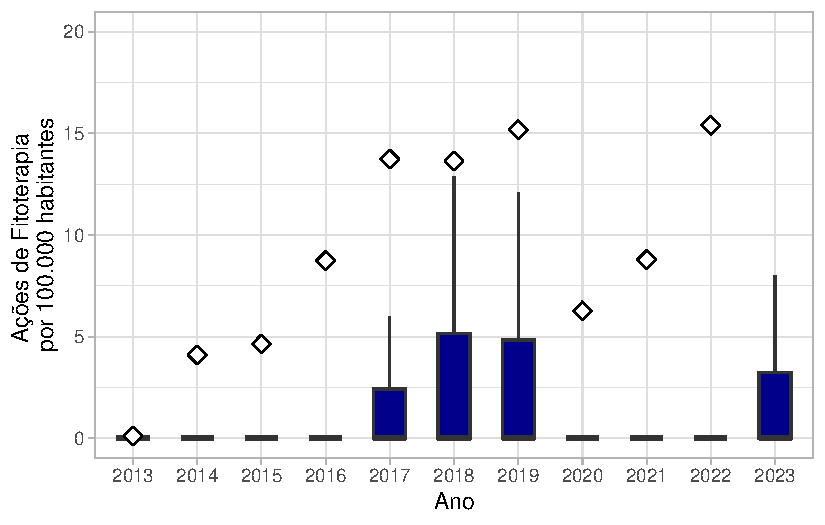
\includegraphics{Relatório_files/figure-pdf/unnamed-chunk-33-1.pdf}

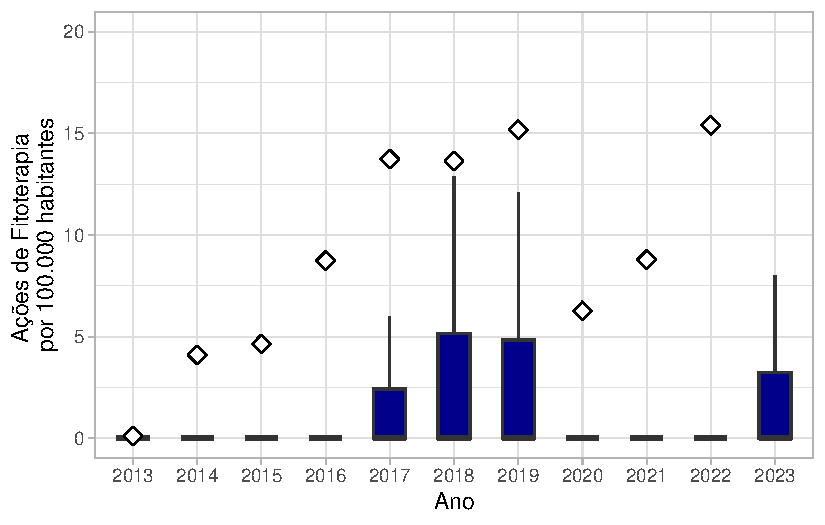
\includegraphics{Relatório_files/figure-pdf/unnamed-chunk-34-1.pdf}

\begin{longtable}[]{@{}
  >{\raggedright\arraybackslash}p{(\columnwidth - 16\tabcolsep) * \real{0.0556}}
  >{\raggedleft\arraybackslash}p{(\columnwidth - 16\tabcolsep) * \real{0.1222}}
  >{\raggedleft\arraybackslash}p{(\columnwidth - 16\tabcolsep) * \real{0.1556}}
  >{\raggedleft\arraybackslash}p{(\columnwidth - 16\tabcolsep) * \real{0.1222}}
  >{\raggedleft\arraybackslash}p{(\columnwidth - 16\tabcolsep) * \real{0.1111}}
  >{\raggedleft\arraybackslash}p{(\columnwidth - 16\tabcolsep) * \real{0.0889}}
  >{\raggedleft\arraybackslash}p{(\columnwidth - 16\tabcolsep) * \real{0.1111}}
  >{\raggedleft\arraybackslash}p{(\columnwidth - 16\tabcolsep) * \real{0.1222}}
  >{\raggedleft\arraybackslash}p{(\columnwidth - 16\tabcolsep) * \real{0.1111}}@{}}
\toprule\noalign{}
\begin{minipage}[b]{\linewidth}\raggedright
ano
\end{minipage} & \begin{minipage}[b]{\linewidth}\raggedleft
média
\end{minipage} & \begin{minipage}[b]{\linewidth}\raggedleft
desvio padrão
\end{minipage} & \begin{minipage}[b]{\linewidth}\raggedleft
máximo
\end{minipage} & \begin{minipage}[b]{\linewidth}\raggedleft
1\_quartil
\end{minipage} & \begin{minipage}[b]{\linewidth}\raggedleft
mediana
\end{minipage} & \begin{minipage}[b]{\linewidth}\raggedleft
3\_quartil
\end{minipage} & \begin{minipage}[b]{\linewidth}\raggedleft
assimetria
\end{minipage} & \begin{minipage}[b]{\linewidth}\raggedleft
curtose
\end{minipage} \\
\midrule\noalign{}
\endhead
\bottomrule\noalign{}
\endlastfoot
2013 & 0.1105979 & 1.229654 & 26.3609 & 0 & 0 & 0.000000 & 14.88685 &
256.3834 \\
2014 & 4.0972436 & 88.166423 & 4079.4608 & 0 & 0 & 0.000000 & 40.45197 &
1748.6897 \\
2015 & 4.6401569 & 67.227493 & 4242.7814 & 0 & 0 & 0.000000 & 56.91099 &
3562.3736 \\
2016 & 8.7366670 & 104.419287 & 6717.7372 & 0 & 0 & 0.000000 & 54.09663
& 3396.1388 \\
2017 & 13.7330032 & 102.897682 & 5147.3823 & 0 & 0 & 2.420800 & 31.38337
& 1351.5453 \\
2018 & 13.6368982 & 70.287624 & 2869.5652 & 0 & 0 & 5.162750 & 19.55926
& 618.3140 \\
2019 & 15.1718024 & 88.807507 & 3865.0307 & 0 & 0 & 4.831250 & 21.55040
& 737.8500 \\
2020 & 6.2654156 & 118.693639 & 5949.1617 & 0 & 0 & 0.000000 & 42.33995
& 1955.7286 \\
2021 & 8.7852121 & 201.410337 & 12222.8231 & 0 & 0 & 0.000000 & 51.85908
& 2936.0999 \\
2022 & 15.4017249 & 247.588820 & 17178.2445 & 0 & 0 & 0.000000 &
62.59911 & 4291.3383 \\
2023 & 25.7724062 & 349.829028 & 24006.5324 & 0 & 0 & 3.244475 &
60.16160 & 4074.9171 \\
\end{longtable}

\begin{longtable}[]{@{}lr@{}}
\caption{10 UFs com maior média de Ações de Fitoterapia por 100.000
habitantes}\tabularnewline
\toprule\noalign{}
UF & Média Ações \\
\midrule\noalign{}
\endfirsthead
\toprule\noalign{}
UF & Média Ações \\
\midrule\noalign{}
\endhead
\bottomrule\noalign{}
\endlastfoot
RS & 52.918075 \\
SC & 22.064663 \\
MG & 17.166434 \\
AL & 16.176861 \\
AM & 11.072779 \\
PE & 8.789596 \\
PI & 8.509932 \\
DF & 8.422411 \\
RN & 6.939926 \\
PB & 6.718420 \\
\end{longtable}

\subsection{Prevenção da
violência}\label{prevenuxe7uxe3o-da-violuxeancia}

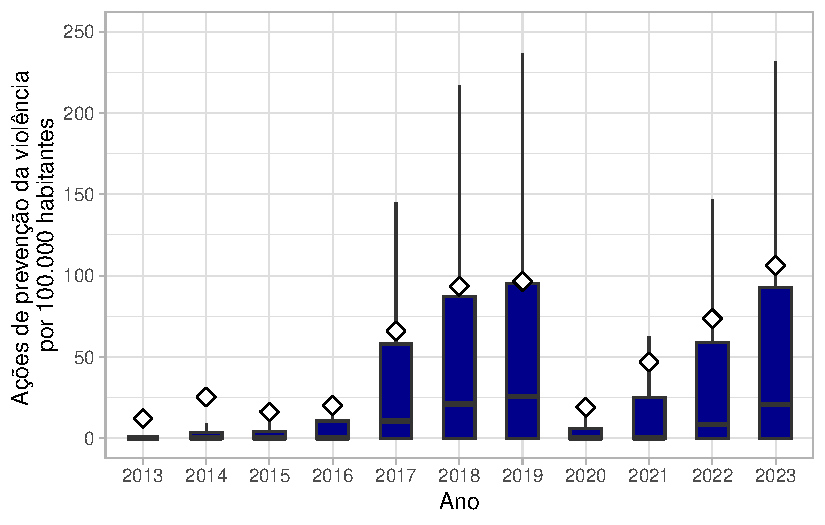
\includegraphics{Relatório_files/figure-pdf/unnamed-chunk-37-1.pdf}

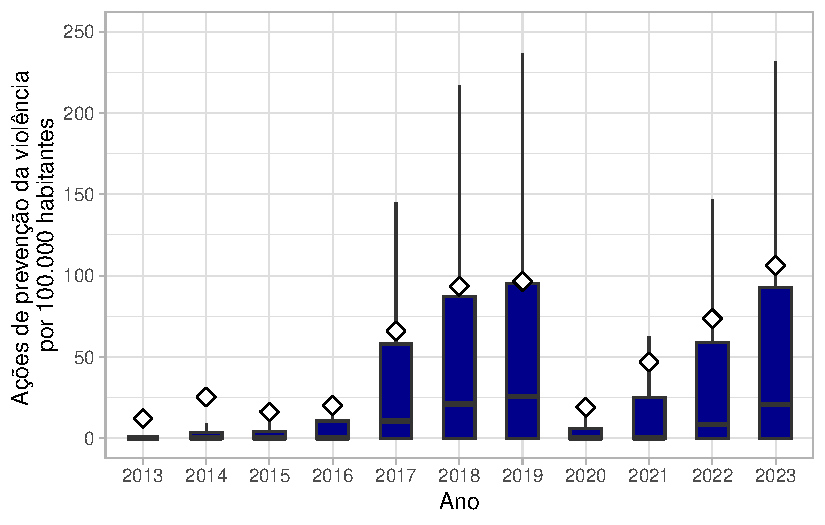
\includegraphics{Relatório_files/figure-pdf/unnamed-chunk-38-1.pdf}

\begin{longtable}[]{@{}
  >{\raggedright\arraybackslash}p{(\columnwidth - 16\tabcolsep) * \real{0.0562}}
  >{\raggedleft\arraybackslash}p{(\columnwidth - 16\tabcolsep) * \real{0.1124}}
  >{\raggedleft\arraybackslash}p{(\columnwidth - 16\tabcolsep) * \real{0.1573}}
  >{\raggedleft\arraybackslash}p{(\columnwidth - 16\tabcolsep) * \real{0.1124}}
  >{\raggedleft\arraybackslash}p{(\columnwidth - 16\tabcolsep) * \real{0.1124}}
  >{\raggedleft\arraybackslash}p{(\columnwidth - 16\tabcolsep) * \real{0.1011}}
  >{\raggedleft\arraybackslash}p{(\columnwidth - 16\tabcolsep) * \real{0.1124}}
  >{\raggedleft\arraybackslash}p{(\columnwidth - 16\tabcolsep) * \real{0.1236}}
  >{\raggedleft\arraybackslash}p{(\columnwidth - 16\tabcolsep) * \real{0.1124}}@{}}
\toprule\noalign{}
\begin{minipage}[b]{\linewidth}\raggedright
ano
\end{minipage} & \begin{minipage}[b]{\linewidth}\raggedleft
média
\end{minipage} & \begin{minipage}[b]{\linewidth}\raggedleft
desvio padrão
\end{minipage} & \begin{minipage}[b]{\linewidth}\raggedleft
máximo
\end{minipage} & \begin{minipage}[b]{\linewidth}\raggedleft
1\_quartil
\end{minipage} & \begin{minipage}[b]{\linewidth}\raggedleft
mediana
\end{minipage} & \begin{minipage}[b]{\linewidth}\raggedleft
3\_quartil
\end{minipage} & \begin{minipage}[b]{\linewidth}\raggedleft
assimetria
\end{minipage} & \begin{minipage}[b]{\linewidth}\raggedleft
curtose
\end{minipage} \\
\midrule\noalign{}
\endhead
\bottomrule\noalign{}
\endlastfoot
2013 & 12.13382 & 80.37185 & 2175.426 & 0 & 0.00000 & 0.00000 & 17.84085
& 436.1704 \\
2014 & 25.34142 & 120.92946 & 2728.972 & 0 & 0.00000 & 3.62350 &
10.86077 & 161.1818 \\
2015 & 16.17345 & 82.44696 & 2879.291 & 0 & 0.00000 & 3.91910 & 16.44759
& 420.7296 \\
2016 & 20.12979 & 77.06046 & 2153.846 & 0 & 0.00000 & 10.54070 &
11.11782 & 198.4289 \\
2017 & 65.96339 & 201.11467 & 5680.990 & 0 & 10.66890 & 57.97100 &
13.04649 & 290.9753 \\
2018 & 93.36469 & 284.64058 & 8641.975 & 0 & 20.90880 & 86.95650 &
12.77444 & 262.5788 \\
2019 & 96.54324 & 261.69497 & 6396.112 & 0 & 25.50530 & 94.96813 &
10.58393 & 175.2281 \\
2020 & 19.10131 & 100.30298 & 4492.754 & 0 & 0.00000 & 6.05545 &
22.61790 & 855.6263 \\
2021 & 46.93658 & 209.75279 & 10672.492 & 0 & 0.00000 & 25.03440 &
28.87442 & 1345.1626 \\
2022 & 73.55115 & 249.92898 & 9585.601 & 0 & 8.56160 & 58.92980 &
15.75103 & 451.9345 \\
2023 & 106.17173 & 359.58529 & 16153.206 & 0 & 20.73615 & 92.73268 &
21.01541 & 785.5325 \\
\end{longtable}

\begin{longtable}[]{@{}lr@{}}
\caption{10 UFs com maior média de Ações de prevenção da violência por
100.000 habitantes}\tabularnewline
\toprule\noalign{}
UF & Média Ações \\
\midrule\noalign{}
\endfirsthead
\toprule\noalign{}
UF & Média Ações \\
\midrule\noalign{}
\endhead
\bottomrule\noalign{}
\endlastfoot
MG & 131.55317 \\
AM & 102.20486 \\
AL & 81.53422 \\
RS & 80.63193 \\
CE & 59.69755 \\
TO & 57.14950 \\
RN & 56.17494 \\
RO & 55.43743 \\
SC & 54.02277 \\
GO & 53.01928 \\
\end{longtable}

\subsection{Saúde ambiental}\label{sauxfade-ambiental}

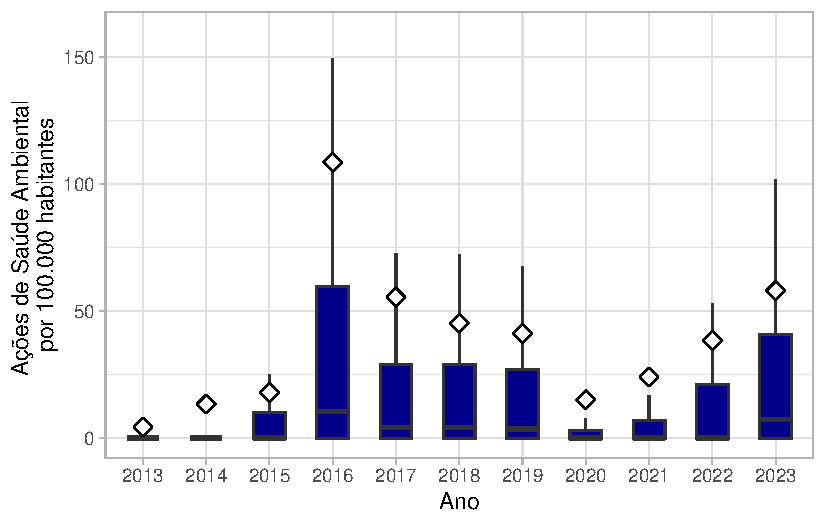
\includegraphics{Relatório_files/figure-pdf/unnamed-chunk-41-1.pdf}

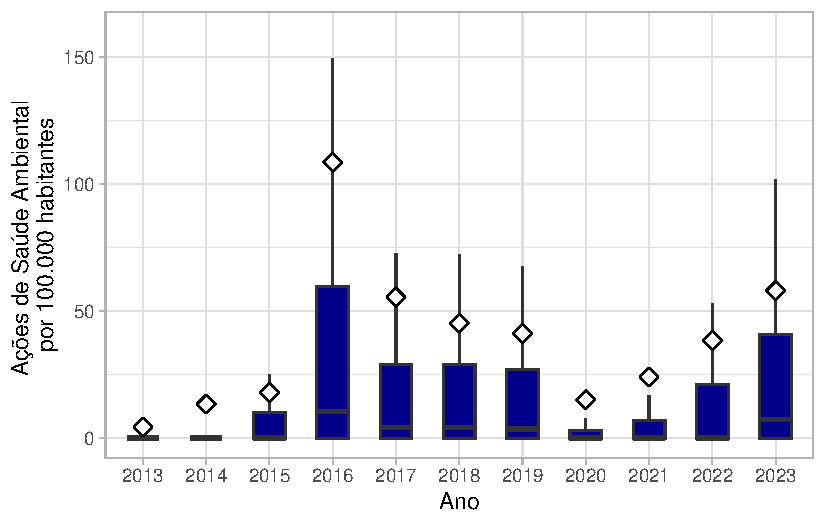
\includegraphics{Relatório_files/figure-pdf/unnamed-chunk-42-1.pdf}

\begin{longtable}[]{@{}
  >{\raggedright\arraybackslash}p{(\columnwidth - 16\tabcolsep) * \real{0.0556}}
  >{\raggedleft\arraybackslash}p{(\columnwidth - 16\tabcolsep) * \real{0.1222}}
  >{\raggedleft\arraybackslash}p{(\columnwidth - 16\tabcolsep) * \real{0.1556}}
  >{\raggedleft\arraybackslash}p{(\columnwidth - 16\tabcolsep) * \real{0.1222}}
  >{\raggedleft\arraybackslash}p{(\columnwidth - 16\tabcolsep) * \real{0.1111}}
  >{\raggedleft\arraybackslash}p{(\columnwidth - 16\tabcolsep) * \real{0.0889}}
  >{\raggedleft\arraybackslash}p{(\columnwidth - 16\tabcolsep) * \real{0.1111}}
  >{\raggedleft\arraybackslash}p{(\columnwidth - 16\tabcolsep) * \real{0.1222}}
  >{\raggedleft\arraybackslash}p{(\columnwidth - 16\tabcolsep) * \real{0.1111}}@{}}
\toprule\noalign{}
\begin{minipage}[b]{\linewidth}\raggedright
ano
\end{minipage} & \begin{minipage}[b]{\linewidth}\raggedleft
média
\end{minipage} & \begin{minipage}[b]{\linewidth}\raggedleft
desvio padrão
\end{minipage} & \begin{minipage}[b]{\linewidth}\raggedleft
máximo
\end{minipage} & \begin{minipage}[b]{\linewidth}\raggedleft
1\_quartil
\end{minipage} & \begin{minipage}[b]{\linewidth}\raggedleft
mediana
\end{minipage} & \begin{minipage}[b]{\linewidth}\raggedleft
3\_quartil
\end{minipage} & \begin{minipage}[b]{\linewidth}\raggedleft
assimetria
\end{minipage} & \begin{minipage}[b]{\linewidth}\raggedleft
curtose
\end{minipage} \\
\midrule\noalign{}
\endhead
\bottomrule\noalign{}
\endlastfoot
2013 & 4.408712 & 35.52339 & 637.7428 & 0 & 0.0000 & 0.00000 & 14.07431
& 229.6713 \\
2014 & 13.423716 & 71.69457 & 2019.0690 & 0 & 0.0000 & 0.00000 &
14.93474 & 316.4935 \\
2015 & 17.933528 & 93.74119 & 4686.4431 & 0 & 0.0000 & 10.13630 &
30.79270 & 1416.9962 \\
2016 & 108.652589 & 785.05743 & 44745.1511 & 0 & 10.5438 & 59.75427 &
40.84350 & 2156.0474 \\
2017 & 55.487578 & 615.48039 & 33964.8173 & 0 & 4.1411 & 29.07670 &
42.09438 & 2039.9427 \\
2018 & 45.237132 & 378.05499 & 23768.1159 & 0 & 4.1417 & 28.98550 &
48.62999 & 2915.3406 \\
2019 & 41.278563 & 240.04656 & 10579.7101 & 0 & 3.6235 & 27.00900 &
26.48451 & 932.2216 \\
2020 & 15.092228 & 103.57037 & 3463.7681 & 0 & 0.0000 & 3.03805 &
18.01452 & 430.6547 \\
2021 & 24.122272 & 141.83460 & 6209.8026 & 0 & 0.0000 & 6.85870 &
24.13661 & 861.3103 \\
2022 & 38.472631 & 186.90477 & 8957.7229 & 0 & 0.0000 & 21.28340 &
25.27496 & 1030.6184 \\
2023 & 58.071595 & 281.05983 & 16194.8376 & 0 & 7.3077 & 40.88210 &
37.59515 & 2033.8338 \\
\end{longtable}

\begin{longtable}[]{@{}lr@{}}
\caption{10 UFs com maior média de Ações de Saúde Ambiental por 100.000
habitantes}\tabularnewline
\toprule\noalign{}
UF & Média Ações \\
\midrule\noalign{}
\endfirsthead
\toprule\noalign{}
UF & Média Ações \\
\midrule\noalign{}
\endhead
\bottomrule\noalign{}
\endlastfoot
RS & 111.10149 \\
AM & 86.41426 \\
AL & 72.39078 \\
MG & 59.33310 \\
MT & 56.78231 \\
GO & 56.60904 \\
RO & 51.34444 \\
TO & 42.09828 \\
AP & 38.48510 \\
SC & 31.69197 \\
\end{longtable}

\subsection{Saúde bucal}\label{sauxfade-bucal}

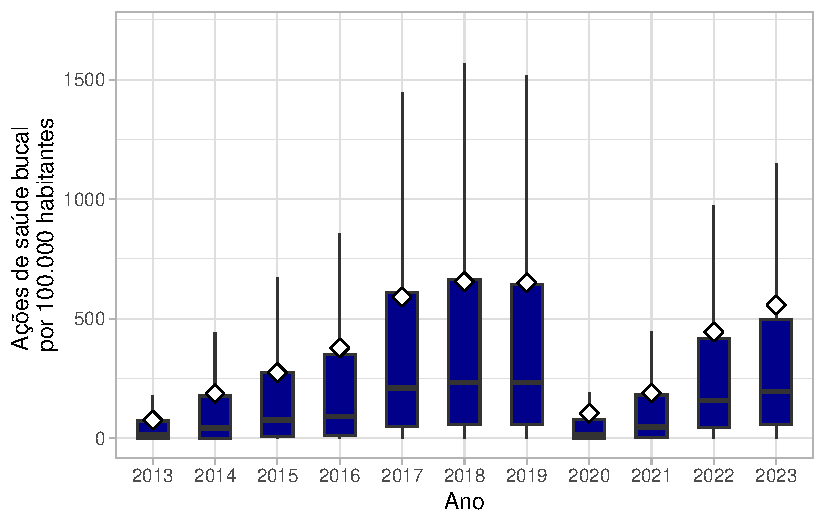
\includegraphics{Relatório_files/figure-pdf/unnamed-chunk-45-1.pdf}

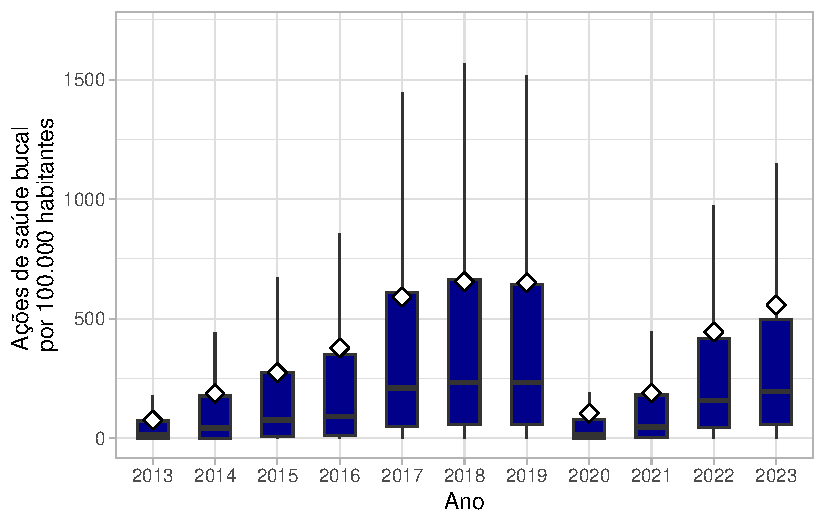
\includegraphics{Relatório_files/figure-pdf/unnamed-chunk-46-1.pdf}

\begin{longtable}[]{@{}
  >{\raggedright\arraybackslash}p{(\columnwidth - 16\tabcolsep) * \real{0.0549}}
  >{\raggedleft\arraybackslash}p{(\columnwidth - 16\tabcolsep) * \real{0.1099}}
  >{\raggedleft\arraybackslash}p{(\columnwidth - 16\tabcolsep) * \real{0.1538}}
  >{\raggedleft\arraybackslash}p{(\columnwidth - 16\tabcolsep) * \real{0.1099}}
  >{\raggedleft\arraybackslash}p{(\columnwidth - 16\tabcolsep) * \real{0.1099}}
  >{\raggedleft\arraybackslash}p{(\columnwidth - 16\tabcolsep) * \real{0.1099}}
  >{\raggedleft\arraybackslash}p{(\columnwidth - 16\tabcolsep) * \real{0.1099}}
  >{\raggedleft\arraybackslash}p{(\columnwidth - 16\tabcolsep) * \real{0.1209}}
  >{\raggedleft\arraybackslash}p{(\columnwidth - 16\tabcolsep) * \real{0.1209}}@{}}
\toprule\noalign{}
\begin{minipage}[b]{\linewidth}\raggedright
ano
\end{minipage} & \begin{minipage}[b]{\linewidth}\raggedleft
média
\end{minipage} & \begin{minipage}[b]{\linewidth}\raggedleft
desvio padrão
\end{minipage} & \begin{minipage}[b]{\linewidth}\raggedleft
máximo
\end{minipage} & \begin{minipage}[b]{\linewidth}\raggedleft
1\_quartil
\end{minipage} & \begin{minipage}[b]{\linewidth}\raggedleft
mediana
\end{minipage} & \begin{minipage}[b]{\linewidth}\raggedleft
3\_quartil
\end{minipage} & \begin{minipage}[b]{\linewidth}\raggedleft
assimetria
\end{minipage} & \begin{minipage}[b]{\linewidth}\raggedleft
curtose
\end{minipage} \\
\midrule\noalign{}
\endhead
\bottomrule\noalign{}
\endlastfoot
2013 & 76.02356 & 187.7854 & 3189.022 & 0.00000 & 13.59815 & 71.89867 &
7.076471 & 84.02165 \\
2014 & 187.14801 & 453.8852 & 8768.116 & 0.00000 & 43.48460 & 176.36680
& 7.991953 & 105.30914 \\
2015 & 274.00375 & 725.6753 & 26110.057 & 7.24875 & 76.18380 & 273.62315
& 14.849030 & 414.71167 \\
2016 & 377.41961 & 1046.8514 & 34005.979 & 11.03378 & 91.91705 &
349.54557 & 12.595404 & 284.87776 \\
2017 & 590.75485 & 1354.9476 & 36338.342 & 48.90980 & 210.64840 &
608.80595 & 9.126902 & 150.37938 \\
2018 & 654.38081 & 1384.8560 & 23246.377 & 57.97380 & 233.64490 &
662.14765 & 6.172215 & 60.17776 \\
2019 & 650.27404 & 1411.1425 & 23066.755 & 57.97940 & 231.88410 &
641.93682 & 6.430160 & 63.61308 \\
2020 & 104.42574 & 443.6831 & 19913.043 & 0.00000 & 15.69490 & 76.84595
& 26.283185 & 1010.17192 \\
2021 & 188.62793 & 470.6670 & 9591.584 & 2.52010 & 47.10320 & 180.97700
& 8.475948 & 115.13346 \\
2022 & 443.80975 & 1018.3263 & 21802.995 & 44.14605 & 158.09730 &
416.32245 & 7.523911 & 90.48632 \\
2023 & 557.13034 & 1355.7120 & 31217.300 & 57.57135 & 194.80680 &
495.27472 & 8.162150 & 109.55009 \\
\end{longtable}

\begin{longtable}[]{@{}lr@{}}
\caption{10 UFs com maior média de Ações de saúde bucal por 100.000
habitantes}\tabularnewline
\toprule\noalign{}
UF & Média Ações \\
\midrule\noalign{}
\endfirsthead
\toprule\noalign{}
UF & Média Ações \\
\midrule\noalign{}
\endhead
\bottomrule\noalign{}
\endlastfoot
PR & 755.8982 \\
AL & 683.7853 \\
SC & 642.7915 \\
MG & 614.6543 \\
TO & 589.5416 \\
RS & 462.4981 \\
MS & 449.5515 \\
MT & 446.5745 \\
AM & 439.4657 \\
PE & 378.4199 \\
\end{longtable}

\subsection{Saúde do trabalhador}\label{sauxfade-do-trabalhador}

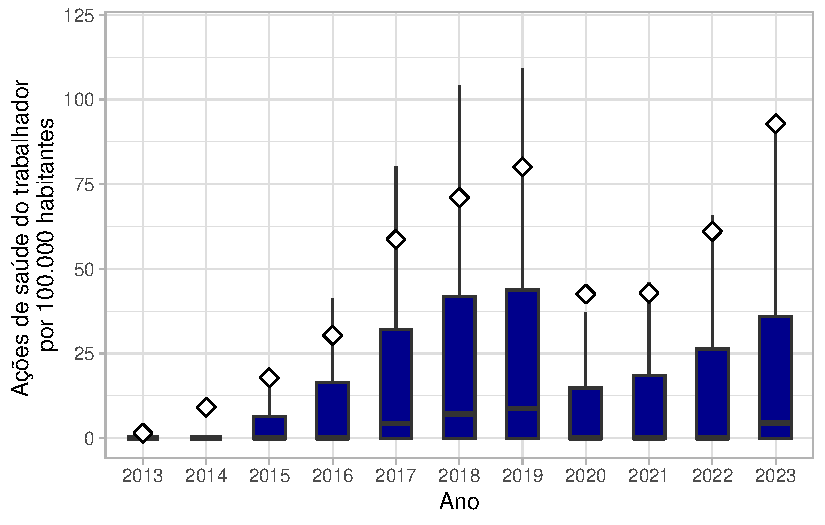
\includegraphics{Relatório_files/figure-pdf/unnamed-chunk-49-1.pdf}

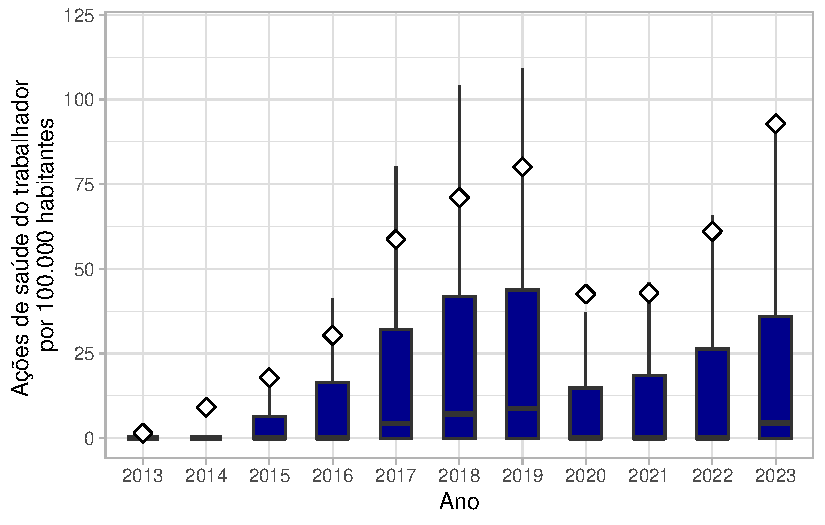
\includegraphics{Relatório_files/figure-pdf/unnamed-chunk-50-1.pdf}

\begin{longtable}[]{@{}
  >{\raggedright\arraybackslash}p{(\columnwidth - 16\tabcolsep) * \real{0.0568}}
  >{\raggedleft\arraybackslash}p{(\columnwidth - 16\tabcolsep) * \real{0.1136}}
  >{\raggedleft\arraybackslash}p{(\columnwidth - 16\tabcolsep) * \real{0.1591}}
  >{\raggedleft\arraybackslash}p{(\columnwidth - 16\tabcolsep) * \real{0.1136}}
  >{\raggedleft\arraybackslash}p{(\columnwidth - 16\tabcolsep) * \real{0.1136}}
  >{\raggedleft\arraybackslash}p{(\columnwidth - 16\tabcolsep) * \real{0.0909}}
  >{\raggedleft\arraybackslash}p{(\columnwidth - 16\tabcolsep) * \real{0.1136}}
  >{\raggedleft\arraybackslash}p{(\columnwidth - 16\tabcolsep) * \real{0.1250}}
  >{\raggedleft\arraybackslash}p{(\columnwidth - 16\tabcolsep) * \real{0.1136}}@{}}
\toprule\noalign{}
\begin{minipage}[b]{\linewidth}\raggedright
ano
\end{minipage} & \begin{minipage}[b]{\linewidth}\raggedleft
média
\end{minipage} & \begin{minipage}[b]{\linewidth}\raggedleft
desvio padrão
\end{minipage} & \begin{minipage}[b]{\linewidth}\raggedleft
máximo
\end{minipage} & \begin{minipage}[b]{\linewidth}\raggedleft
1\_quartil
\end{minipage} & \begin{minipage}[b]{\linewidth}\raggedleft
mediana
\end{minipage} & \begin{minipage}[b]{\linewidth}\raggedleft
3\_quartil
\end{minipage} & \begin{minipage}[b]{\linewidth}\raggedleft
assimetria
\end{minipage} & \begin{minipage}[b]{\linewidth}\raggedleft
curtose
\end{minipage} \\
\midrule\noalign{}
\endhead
\bottomrule\noalign{}
\endlastfoot
2013 & 1.488605 & 29.95387 & 1028.383 & 0 & 0.0000 & 0.00000 & 32.66286
& 1113.4485 \\
2014 & 9.153506 & 70.99049 & 1814.493 & 0 & 0.0000 & 0.00000 & 16.76129
& 355.5723 \\
2015 & 17.841975 & 115.77676 & 4278.075 & 0 & 0.0000 & 6.44225 &
21.34294 & 607.2915 \\
2016 & 30.339019 & 150.00907 & 5128.205 & 0 & 0.0000 & 16.44335 &
17.01745 & 416.7447 \\
2017 & 58.713908 & 263.36628 & 5597.068 & 0 & 4.3264 & 32.08885 &
12.16694 & 190.0587 \\
2018 & 71.049001 & 306.01581 & 9096.972 & 0 & 7.1235 & 41.76100 &
13.56702 & 270.0549 \\
2019 & 80.112241 & 363.55914 & 10160.428 & 0 & 8.6954 & 43.73342 &
13.42932 & 248.4480 \\
2020 & 42.551882 & 240.86031 & 9710.145 & 0 & 0.0000 & 14.84175 &
20.08988 & 620.5510 \\
2021 & 42.823653 & 240.33636 & 10610.080 & 0 & 0.0000 & 18.39780 &
23.54084 & 845.2713 \\
2022 & 61.072691 & 339.06583 & 12140.763 & 0 & 0.0000 & 26.33830 &
17.64310 & 443.2371 \\
2023 & 92.809989 & 632.17439 & 27187.916 & 0 & 4.4657 & 35.99063 &
24.28618 & 812.0230 \\
\end{longtable}

\begin{longtable}[]{@{}lr@{}}
\caption{10 UFs com maior média de Ações de saúde do trabalhador por
100.000 habitantes}\tabularnewline
\toprule\noalign{}
UF & Média Ações \\
\midrule\noalign{}
\endfirsthead
\toprule\noalign{}
UF & Média Ações \\
\midrule\noalign{}
\endhead
\bottomrule\noalign{}
\endlastfoot
MG & 145.58411 \\
AM & 76.84984 \\
RS & 65.26777 \\
TO & 62.38343 \\
GO & 59.79504 \\
SC & 58.33461 \\
AL & 51.29654 \\
RN & 40.75957 \\
MT & 37.68109 \\
MS & 35.90552 \\
\end{longtable}

\subsection{Saúde mental}\label{sauxfade-mental}

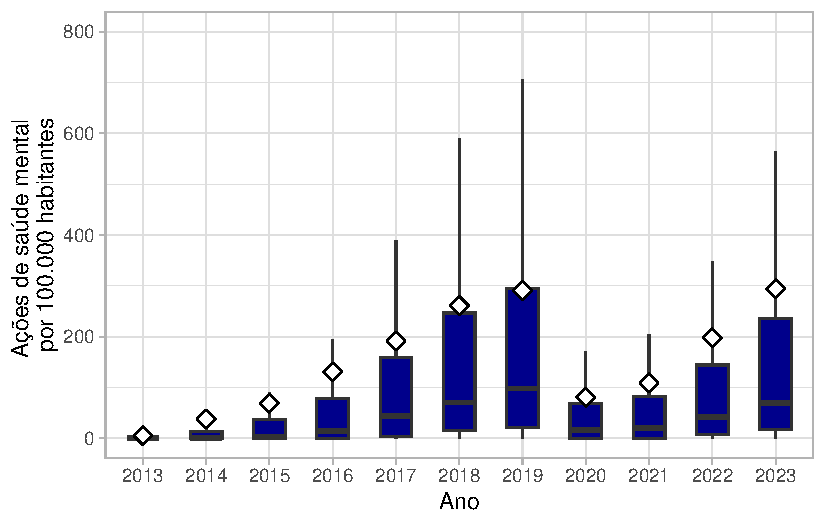
\includegraphics{Relatório_files/figure-pdf/unnamed-chunk-53-1.pdf}

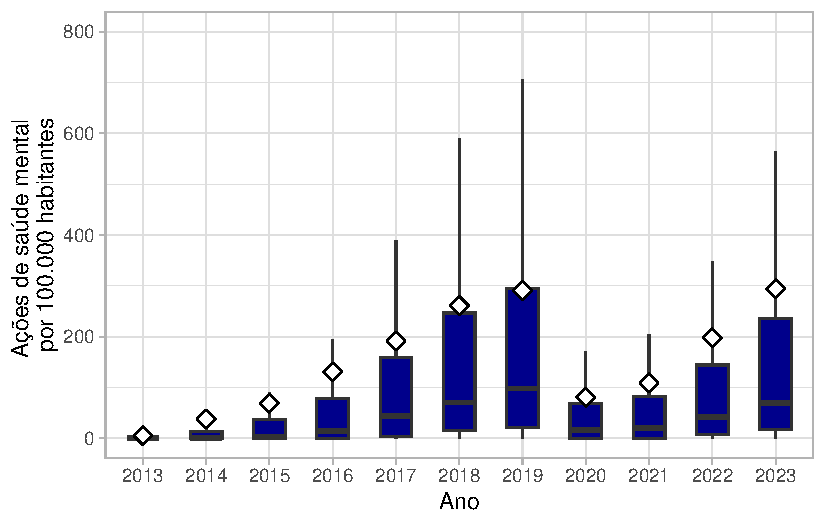
\includegraphics{Relatório_files/figure-pdf/unnamed-chunk-54-1.pdf}

\begin{longtable}[]{@{}
  >{\raggedright\arraybackslash}p{(\columnwidth - 16\tabcolsep) * \real{0.0549}}
  >{\raggedleft\arraybackslash}p{(\columnwidth - 16\tabcolsep) * \real{0.1209}}
  >{\raggedleft\arraybackslash}p{(\columnwidth - 16\tabcolsep) * \real{0.1538}}
  >{\raggedleft\arraybackslash}p{(\columnwidth - 16\tabcolsep) * \real{0.1209}}
  >{\raggedleft\arraybackslash}p{(\columnwidth - 16\tabcolsep) * \real{0.1099}}
  >{\raggedleft\arraybackslash}p{(\columnwidth - 16\tabcolsep) * \real{0.0879}}
  >{\raggedleft\arraybackslash}p{(\columnwidth - 16\tabcolsep) * \real{0.1099}}
  >{\raggedleft\arraybackslash}p{(\columnwidth - 16\tabcolsep) * \real{0.1209}}
  >{\raggedleft\arraybackslash}p{(\columnwidth - 16\tabcolsep) * \real{0.1209}}@{}}
\toprule\noalign{}
\begin{minipage}[b]{\linewidth}\raggedright
ano
\end{minipage} & \begin{minipage}[b]{\linewidth}\raggedleft
média
\end{minipage} & \begin{minipage}[b]{\linewidth}\raggedleft
desvio padrão
\end{minipage} & \begin{minipage}[b]{\linewidth}\raggedleft
máximo
\end{minipage} & \begin{minipage}[b]{\linewidth}\raggedleft
1\_quartil
\end{minipage} & \begin{minipage}[b]{\linewidth}\raggedleft
mediana
\end{minipage} & \begin{minipage}[b]{\linewidth}\raggedleft
3\_quartil
\end{minipage} & \begin{minipage}[b]{\linewidth}\raggedleft
assimetria
\end{minipage} & \begin{minipage}[b]{\linewidth}\raggedleft
curtose
\end{minipage} \\
\midrule\noalign{}
\endhead
\bottomrule\noalign{}
\endlastfoot
2013 & 5.155549 & 42.29574 & 942.8403 & 0.00000 & 0.0000 & 0.00000 &
17.623152 & 360.48579 \\
2014 & 37.665100 & 224.38387 & 9338.0615 & 0.00000 & 0.0000 & 13.17520 &
27.937682 & 1071.11511 \\
2015 & 68.841282 & 244.91981 & 6619.3853 & 0.00000 & 2.8988 & 36.23450 &
9.844657 & 164.24504 \\
2016 & 130.444345 & 431.34604 & 7060.1419 & 0.00000 & 14.4928 & 77.40295
& 7.894791 & 87.35046 \\
2017 & 191.472147 & 512.54122 & 11249.6376 & 3.83800 & 43.4825 &
158.24880 & 8.388341 & 116.22173 \\
2018 & 261.123823 & 678.18976 & 20434.7826 & 14.49280 & 70.3963 &
246.32755 & 11.197487 & 225.93993 \\
2019 & 290.960285 & 658.32096 & 14053.8786 & 20.70480 & 97.6088 &
295.17638 & 8.281878 & 113.54911 \\
2020 & 80.625519 & 233.64052 & 5863.8743 & 0.00000 & 15.7629 & 67.97520
& 10.058110 & 158.90445 \\
2021 & 108.959838 & 421.34358 & 16203.7037 & 0.00000 & 19.9641 &
81.71600 & 19.987019 & 607.40244 \\
2022 & 197.659795 & 804.65988 & 41062.3557 & 7.27470 & 41.8410 &
143.87415 & 27.798683 & 1268.39106 \\
2023 & 294.183177 & 934.84546 & 28637.4134 & 17.18708 & 69.4525 &
235.98638 & 13.842598 & 307.95344 \\
\end{longtable}

\begin{longtable}[]{@{}lr@{}}
\caption{10 UFs com maior média de Ações de saúde mental por 100.000
habitantes}\tabularnewline
\toprule\noalign{}
UF & Média Ações \\
\midrule\noalign{}
\endfirsthead
\toprule\noalign{}
UF & Média Ações \\
\midrule\noalign{}
\endhead
\bottomrule\noalign{}
\endlastfoot
RS & 434.1025 \\
MG & 262.7377 \\
SC & 243.8555 \\
GO & 193.1804 \\
SP & 162.2464 \\
AL & 152.2775 \\
TO & 150.9871 \\
MT & 146.2468 \\
AM & 141.2209 \\
PR & 120.5919 \\
\end{longtable}

\subsection{Saúde sexual e
reprodutiva}\label{sauxfade-sexual-e-reprodutiva}

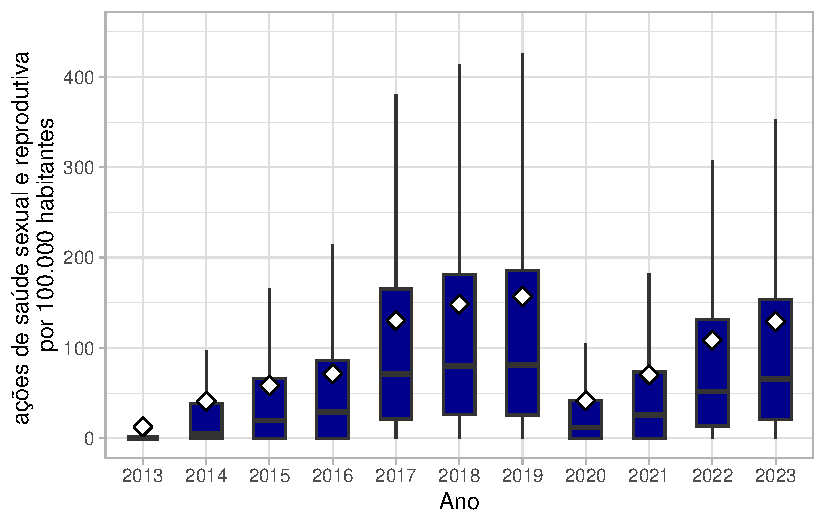
\includegraphics{Relatório_files/figure-pdf/unnamed-chunk-57-1.pdf}

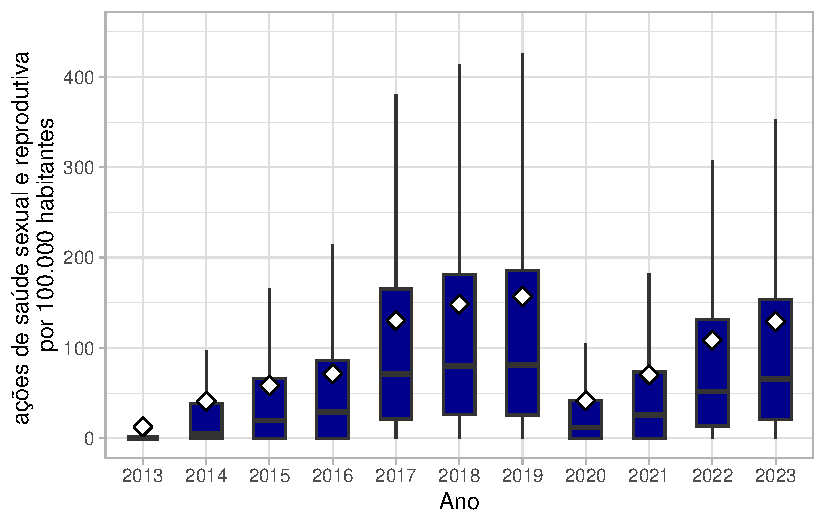
\includegraphics{Relatório_files/figure-pdf/unnamed-chunk-58-1.pdf}

\begin{longtable}[]{@{}
  >{\raggedright\arraybackslash}p{(\columnwidth - 16\tabcolsep) * \real{0.0575}}
  >{\raggedleft\arraybackslash}p{(\columnwidth - 16\tabcolsep) * \real{0.1149}}
  >{\raggedleft\arraybackslash}p{(\columnwidth - 16\tabcolsep) * \real{0.1609}}
  >{\raggedleft\arraybackslash}p{(\columnwidth - 16\tabcolsep) * \real{0.1034}}
  >{\raggedleft\arraybackslash}p{(\columnwidth - 16\tabcolsep) * \real{0.1149}}
  >{\raggedleft\arraybackslash}p{(\columnwidth - 16\tabcolsep) * \real{0.0920}}
  >{\raggedleft\arraybackslash}p{(\columnwidth - 16\tabcolsep) * \real{0.1149}}
  >{\raggedleft\arraybackslash}p{(\columnwidth - 16\tabcolsep) * \real{0.1264}}
  >{\raggedleft\arraybackslash}p{(\columnwidth - 16\tabcolsep) * \real{0.1149}}@{}}
\toprule\noalign{}
\begin{minipage}[b]{\linewidth}\raggedright
ano
\end{minipage} & \begin{minipage}[b]{\linewidth}\raggedleft
média
\end{minipage} & \begin{minipage}[b]{\linewidth}\raggedleft
desvio padrão
\end{minipage} & \begin{minipage}[b]{\linewidth}\raggedleft
máximo
\end{minipage} & \begin{minipage}[b]{\linewidth}\raggedleft
1\_quartil
\end{minipage} & \begin{minipage}[b]{\linewidth}\raggedleft
mediana
\end{minipage} & \begin{minipage}[b]{\linewidth}\raggedleft
3\_quartil
\end{minipage} & \begin{minipage}[b]{\linewidth}\raggedleft
assimetria
\end{minipage} & \begin{minipage}[b]{\linewidth}\raggedleft
curtose
\end{minipage} \\
\midrule\noalign{}
\endhead
\bottomrule\noalign{}
\endlastfoot
2013 & 12.57458 & 56.41209 & 1160.227 & 0.00000 & 0.0000 & 0.00000 &
11.414224 & 183.59304 \\
2014 & 40.95282 & 102.71198 & 1495.314 & 0.00000 & 4.8816 & 38.65110 &
6.914625 & 75.13960 \\
2015 & 58.35415 & 117.84364 & 1785.714 & 0.00000 & 19.3259 & 66.42075 &
5.656654 & 53.03156 \\
2016 & 71.41506 & 127.87216 & 1906.234 & 0.00000 & 28.9876 & 85.98450 &
4.929554 & 41.52680 \\
2017 & 130.11853 & 198.64664 & 3205.495 & 21.37490 & 70.8717 & 165.15120
& 5.140748 & 49.24246 \\
2018 & 148.27293 & 233.75058 & 4724.638 & 25.89290 & 79.7159 & 181.22730
& 6.107079 & 73.73714 \\
2019 & 156.79445 & 254.69023 & 3630.728 & 25.76800 & 81.2297 & 185.85350
& 5.190048 & 45.95195 \\
2020 & 41.65230 & 107.62549 & 3045.685 & 0.00000 & 11.6822 & 42.02565 &
11.522535 & 237.65703 \\
2021 & 70.19145 & 156.70156 & 3342.689 & 0.00000 & 25.9213 & 73.17070 &
7.778850 & 100.51522 \\
2022 & 108.38301 & 181.42919 & 3310.475 & 13.56115 & 51.6396 & 131.07880
& 5.706863 & 63.51086 \\
2023 & 129.16338 & 239.70999 & 7171.854 & 20.66118 & 65.7462 & 153.62592
& 11.480189 & 255.46231 \\
\end{longtable}

\begin{longtable}[]{@{}lr@{}}
\caption{10 UFs com maior média de ações de saúde sexual e reprodutiva
por 100.000 habitantes}\tabularnewline
\toprule\noalign{}
UF & Média Ações \\
\midrule\noalign{}
\endfirsthead
\toprule\noalign{}
UF & Média Ações \\
\midrule\noalign{}
\endhead
\bottomrule\noalign{}
\endlastfoot
AL & 237.6767 \\
AM & 204.2715 \\
TO & 135.2094 \\
MG & 127.6155 \\
CE & 120.7105 \\
PE & 118.5709 \\
RN & 117.0914 \\
RO & 110.5853 \\
PA & 109.5711 \\
PB & 108.8567 \\
\end{longtable}

\subsection{Semana saúde na escola}\label{semana-sauxfade-na-escola}

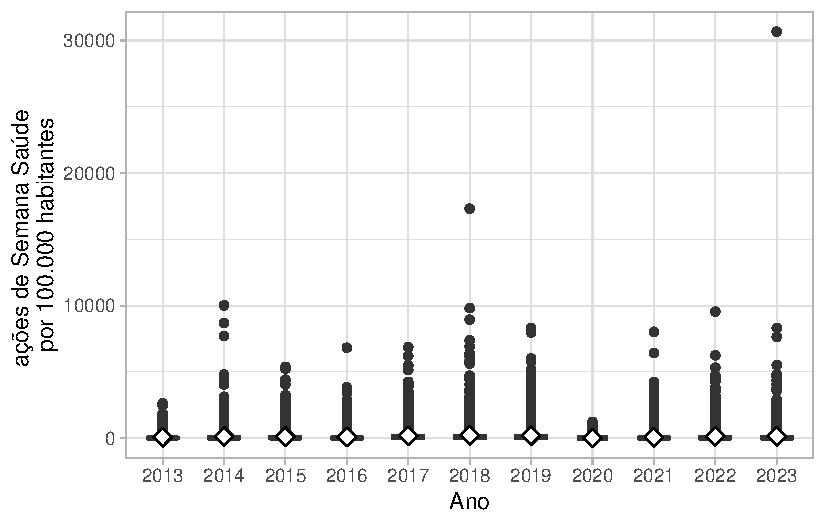
\includegraphics{Relatório_files/figure-pdf/unnamed-chunk-61-1.pdf}

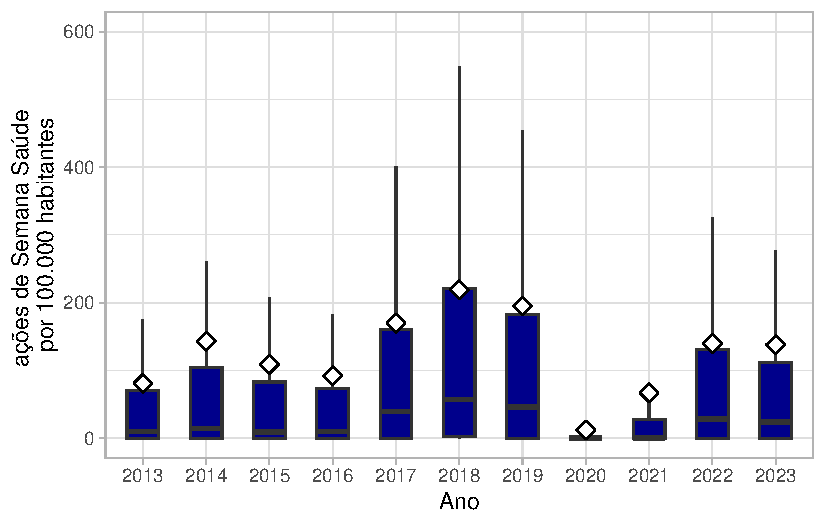
\includegraphics{Relatório_files/figure-pdf/unnamed-chunk-62-1.pdf}

\begin{longtable}[]{@{}
  >{\raggedright\arraybackslash}p{(\columnwidth - 16\tabcolsep) * \real{0.0556}}
  >{\raggedleft\arraybackslash}p{(\columnwidth - 16\tabcolsep) * \real{0.1111}}
  >{\raggedleft\arraybackslash}p{(\columnwidth - 16\tabcolsep) * \real{0.1556}}
  >{\raggedleft\arraybackslash}p{(\columnwidth - 16\tabcolsep) * \real{0.1111}}
  >{\raggedleft\arraybackslash}p{(\columnwidth - 16\tabcolsep) * \real{0.1111}}
  >{\raggedleft\arraybackslash}p{(\columnwidth - 16\tabcolsep) * \real{0.1000}}
  >{\raggedleft\arraybackslash}p{(\columnwidth - 16\tabcolsep) * \real{0.1111}}
  >{\raggedleft\arraybackslash}p{(\columnwidth - 16\tabcolsep) * \real{0.1222}}
  >{\raggedleft\arraybackslash}p{(\columnwidth - 16\tabcolsep) * \real{0.1222}}@{}}
\toprule\noalign{}
\begin{minipage}[b]{\linewidth}\raggedright
ano
\end{minipage} & \begin{minipage}[b]{\linewidth}\raggedleft
média
\end{minipage} & \begin{minipage}[b]{\linewidth}\raggedleft
desvio padrão
\end{minipage} & \begin{minipage}[b]{\linewidth}\raggedleft
máximo
\end{minipage} & \begin{minipage}[b]{\linewidth}\raggedleft
1\_quartil
\end{minipage} & \begin{minipage}[b]{\linewidth}\raggedleft
mediana
\end{minipage} & \begin{minipage}[b]{\linewidth}\raggedleft
3\_quartil
\end{minipage} & \begin{minipage}[b]{\linewidth}\raggedleft
assimetria
\end{minipage} & \begin{minipage}[b]{\linewidth}\raggedleft
curtose
\end{minipage} \\
\midrule\noalign{}
\endhead
\bottomrule\noalign{}
\endlastfoot
2013 & 80.85779 & 223.6116 & 2637.194 & 0.00000 & 9.66180 & 70.12743 &
6.700608 & 62.48315 \\
2014 & 143.00021 & 456.2149 & 10020.638 & 0.00000 & 14.60920 & 104.64630
& 10.403942 & 167.74568 \\
2015 & 109.13668 & 310.6868 & 5377.608 & 0.00000 & 8.92780 & 82.90855 &
7.009035 & 75.45433 \\
2016 & 92.00186 & 256.7591 & 6822.430 & 0.00000 & 9.66195 & 72.82438 &
8.404575 & 134.70444 \\
2017 & 169.79386 & 393.4604 & 6865.742 & 0.00000 & 39.66680 & 160.35275
& 6.106383 & 61.12264 \\
2018 & 219.30422 & 549.2611 & 17313.359 & 2.36735 & 57.16900 & 220.74220
& 10.929794 & 232.99159 \\
2019 & 195.18067 & 467.8085 & 8310.992 & 0.00000 & 45.90130 & 182.33180
& 6.530663 & 67.66586 \\
2020 & 12.04586 & 57.3330 & 1226.054 & 0.00000 & 0.00000 & 0.00000 &
9.230783 & 119.42283 \\
2021 & 67.02653 & 276.3130 & 8025.478 & 0.00000 & 0.00000 & 27.13700 &
12.348634 & 244.84385 \\
2022 & 139.75392 & 355.4877 & 9544.159 & 0.00000 & 28.39300 & 130.96415
& 8.967657 & 149.05271 \\
2023 & 137.99332 & 548.5710 & 30659.226 & 0.00000 & 23.88350 & 111.26212
& 34.151720 & 1788.96604 \\
\end{longtable}

\begin{longtable}[]{@{}lr@{}}
\caption{10 UFs com maior média de ações de Semana Saúde por 100.000
habitantes}\tabularnewline
\toprule\noalign{}
UF & Média Ações \\
\midrule\noalign{}
\endfirsthead
\toprule\noalign{}
UF & Média Ações \\
\midrule\noalign{}
\endhead
\bottomrule\noalign{}
\endlastfoot
AM & 205.5722 \\
RN & 205.5154 \\
AL & 198.1576 \\
TO & 189.9257 \\
PB & 184.4466 \\
MG & 173.0704 \\
MT & 159.9126 \\
SC & 153.7059 \\
PI & 130.7770 \\
PE & 127.2492 \\
\end{longtable}




\end{document}
